\chapter{A utility class for aircraft modeling: \texttt{AircraftUtils}}
\label{chap3}

\section{Introduction}
\label{sec3.1}

Once the \lstinline[language=Java]!JPADCAD! library was developed, providing basic methods for the construction of \gls{CAD} shapes, these same methods have been used to create functions that, starting from the geometric characteristics of a given aeronautical component supplied in input, automatically generate the \gls{CAD} model of the aircraft, complete of all of its components or just a given number of them. As stated in Chapter \ref{chap1}, \gls{JPAD} comes equipped with classes and methods that allow to read data regarding the aircraft and its components from appropriately formatted XML files. Reading this data determines the creation of an instance of the \gls{JPAD} \lstinline[language=Java]!Aircraft! class. This class is the one delegated to the storage of all the data related to the aircraft, and also contains all the methods that allow access to the different sub-components of the airplane. These sub-components are treated in \gls{JPAD} by the use of different classes. As for the sub-components currently modeled through the use of \lstinline[language=Java]!JPADCAD!, the \lstinline[language=Java]!Fuselage! and \lstinline[language=Java]!LiftingSurface! classes are those delegated to the description, respectively, of the fuselage and all the different types of aerodynamic components in general. For this reason, the \lstinline[language=Java]!LiftingSurface! class can be used, for example, to describe both wings and tail surfaces. The modeling of the \gls{CAD} entities of the different components of an aircraft starts from the instances of these classes, as it will be more evident in the next paragraphs.

\section{\texttt{AircraftUtils} overview}
\label{sec3.2}

In order to develop and test methods allowing the construction, from scratch, of aircraft principal components, a new package has been added to the \gls{JPAD} three. This package, named \lstinline[language=Java]!JPADCADSandbox!, has been conceived with the intent to build some sort of \emph{playground} for all the activities inherent to \gls{CAD} modeling. For this reason, this package not only contains the test classes produced to check the correct functioning of the methods contained in \lstinline[language=Java]!JPADCAD!. On the contrary, at present, it also contains all the methods used to build the 3D counterparts of the instances of the \lstinline[language=Java]!Fuselage! and \lstinline[language=Java]!LiftingSurface! classes. These methods have all been collected in one class, along with others that will be listed in the following, which serves as an utility class, i.e., a class that does not need to be instantiated and provides several methods for multiple other classes. These methods can then be accessed in a static way, providing an approach to the solution of a problem which is not properly object oriented (like should be when using a programming language such as Java), but that produces easy to debug/mantain code, which is an important prerequisite especially when developing new functionalities. This utility class is called \lstinline[language=Java]!AircraftUtils! and, along with the methods that have been referred very briefly above, it also provides functions that can be used to:
%
\begin{itemize}
\item load an aircraft from XML file;
\item write aircraft solid components to file;
\item get the whole aircraft shapes.
\end{itemize}
%
All these methods are set to public, meaning that they can be actually accessed by external classes. Furthermore, \lstinline[language=Java]!AircraftUtils! contains several private methods (i.e., functions that can be used only by classes and methods internal to the class in which they are defined), that provide support when dealing, for example, with the wing tip building. Finally, it also includes some enumeration classes, dealing with file extension and spacing type. These enumerators are mainly used internally \lstinline[language=Java]!AircraftUtils!, and more will be said about them and all the public extra methods in paragraph \ref{sec3.5}. 

\bigskip
\noindent
The next two paragraphs, instead, deal with the methodologies and the functions used to build main aircraft components: the fuselage and the lifting surfaces. In order to build these components properly, some sort of construction strategy must be followed. This is a crucial point, especially when dealing with the necessity of using the same code for the construction of the most various shapes and configurations. For this reason, the typical modeling strategies for aircraft geometric design were adopted \cite{paperCADinAero}, by making use of all the primary functions generally used when dealing with object such as fuselages and wings. Classically, typical aircraft components are modeled by means of loft functions. This type of functions, that have been described in paragraph \ref{sec2.3.2} along with their implementation in \lstinline[language=Java]!JPADCAD!, usually requires planar section curves, plus guide curves in some cases (actually not the underlyng \gls{OCCT} algorithm used for the \lstinline[language=Java]!ThruSections! methods), to build shapes that could not be obtained by use of simple extrude, revolve or sweep functions. When dealing with aircraft geometric modeling, loft functions are undoubtedly the most used ones. In order to actually use these functions, it is necessary to construct a wireframe first. This wireframe consists of a set of primary shapes (basically curves or wires) that helps building the final 3D model and provides a first glimpse at the result we coming up with. In aircraft modeling, two different types of primary shapes exist: wing-type shapes and fuselage-type shapes. In case of wing-type shapes the defining sections are parallel to the flow direction and are tipically airfoils, while in case of fuselage-type shapes the defining sections are normal to the flow direction and are symmetrical. Once the wireframes have been defined lofting operations can begin, giving life to the succession of steps that will lead to the generation of the definitive 3D model of the aeronautical component. The methods described below, which return the shapes of primary aircraft components, follow the just described methodology. The next paragraphs therefore provide a focus on how these steps are followed and which classes and methods the construction functions make use of. Moreover, when explaining the algorithms behind the creation of the 3D model of a lifitng surface, a particular emphasis will be given to the methodology followed for the generation of the wing tip, which is the element of greater complexity of the 3D wing produced by \gls{JPAD}. 

\section{Fuselage CAD method}
\label{sec3.3}

In order to help the subsequent lofting operations, it was first necessary to conceive a subdivision of the surface of the fuselage. Thankfully \gls{JPAD} \lstinline[language=Java]!Fuselage! class helps doing this by providing a schematization of the external surface which can be easily used for \gls{CAD} purposes. This scheme splits the fuselage in five principal parts, which can be listed as follows:
%
\begin{itemize}
\item nose cap,
\item nose trunk,
\item cylindrical trunk,
\item tail trunk,
\item tail cap.
\end{itemize}
%
When coming to the \gls{CAD} generation problem, one could imagine each of the parts mentioned above having its own patch being produced by means of a lofting method. The union of these patches (obtained by the use of sewing algorithms) determines the final shape of the fuselage (figure \ref{fig:FusInfographic}). This subdivision not only helps building lofts representing the external surface, making the patching through sections phase much easier. It also provides an useful scheme that has been actually used to fix the parameters of the algorithm for the fuselage construction. The method doing this is called \lstinline[language=Java]!getFuselageCAD! and the parameters it accepts are the followings.
%
\begin{itemize}
\renewcommand\labelitemi{\tiny$\blacksquare$}
\renewcommand\labelitemii{\tiny$\bullet$}
\item \textbf{\lstinline[language=Java]!fuselage!} - An instance of the \lstinline[language=Java]!Fuselage! type containing all the geometric information about the component. It provides easy access to the lists of points defining side curves and outlines. It also contains methods returning the $x$-coordinates of the sections delimiting one part of the fuselage from another.
\item \textbf{\lstinline[language=Java]!noseCapSectionFactor1!, \lstinline[language=Java]!noseCapSectionFactor2!} - Entries defining the limits, in terms of $x$-coordinates, of the nose cap patch. In particular, these factors (which are expressed as Java \lstinline[language=Java]!double!) multiply the nose cap offset length normalized with respect to the nose length, thus returning the normalized initial and terminal $x$-coordinates of the sections defining the shape of the nose cap. 
\item \textbf{\lstinline[language=Java]!numberNoseCapSections!} - An \lstinline[language=Java]!int! fixing the number of nose cap sections to patch through. 
\item \textbf{\lstinline[language=Java]!numberNosePatchSections!} - An \lstinline[language=Java]!int! defining the number of nose trunk sections.
\item \textbf{\lstinline[language=Java]!spacingTypeNosePatch!} - An instance of one of the Java \lstinline[language=Java]!enum! classes mentioned above, defining the type of spacing to be adopted for the sections of the nose trunk. 
\item \textbf{\lstinline[language=Java]!numberTailPatchSections!} - An \lstinline[language=Java]!int! value defining the number of sections to be created for the tail trunk.
\item \textbf{\lstinline[language=Java]!spacingTypeTailPatch!} - The spacing type for the tail trunk sections.
\item \textbf{\lstinline[language=Java]!tailCapSectionFactor1!, \lstinline[language=Java]!tailCapSectionFactor2!} - What has been said for the nose cap sections applies here. These factors simply fix the $x$-coordinates of the tail cap initial and terminal sections.
\item \textbf{\lstinline[language=Java]!numberTailCapSections!} - An \lstinline[language=Java]!int! value fixing the number of tail cap sections to patch through.
\item \textbf{\lstinline[language=Java]!exportSupportShapes!, \lstinline[language=Java]!exportLofts!, \lstinline[language=Java]!exportSolids!} - Entries of the Java \lstinline[language=Java]!boolean! type, allowing the user to select which kind of shapes he wants to generate and export, with the shapes being respectively: support shapes, such as those defining the wireframe of the fuselage; loft shapes, generated by patching through the fuselage sections; solid shapes, obtained by sewing the lofts.
\end{itemize}
%
\begin{figure}[H]
\centering
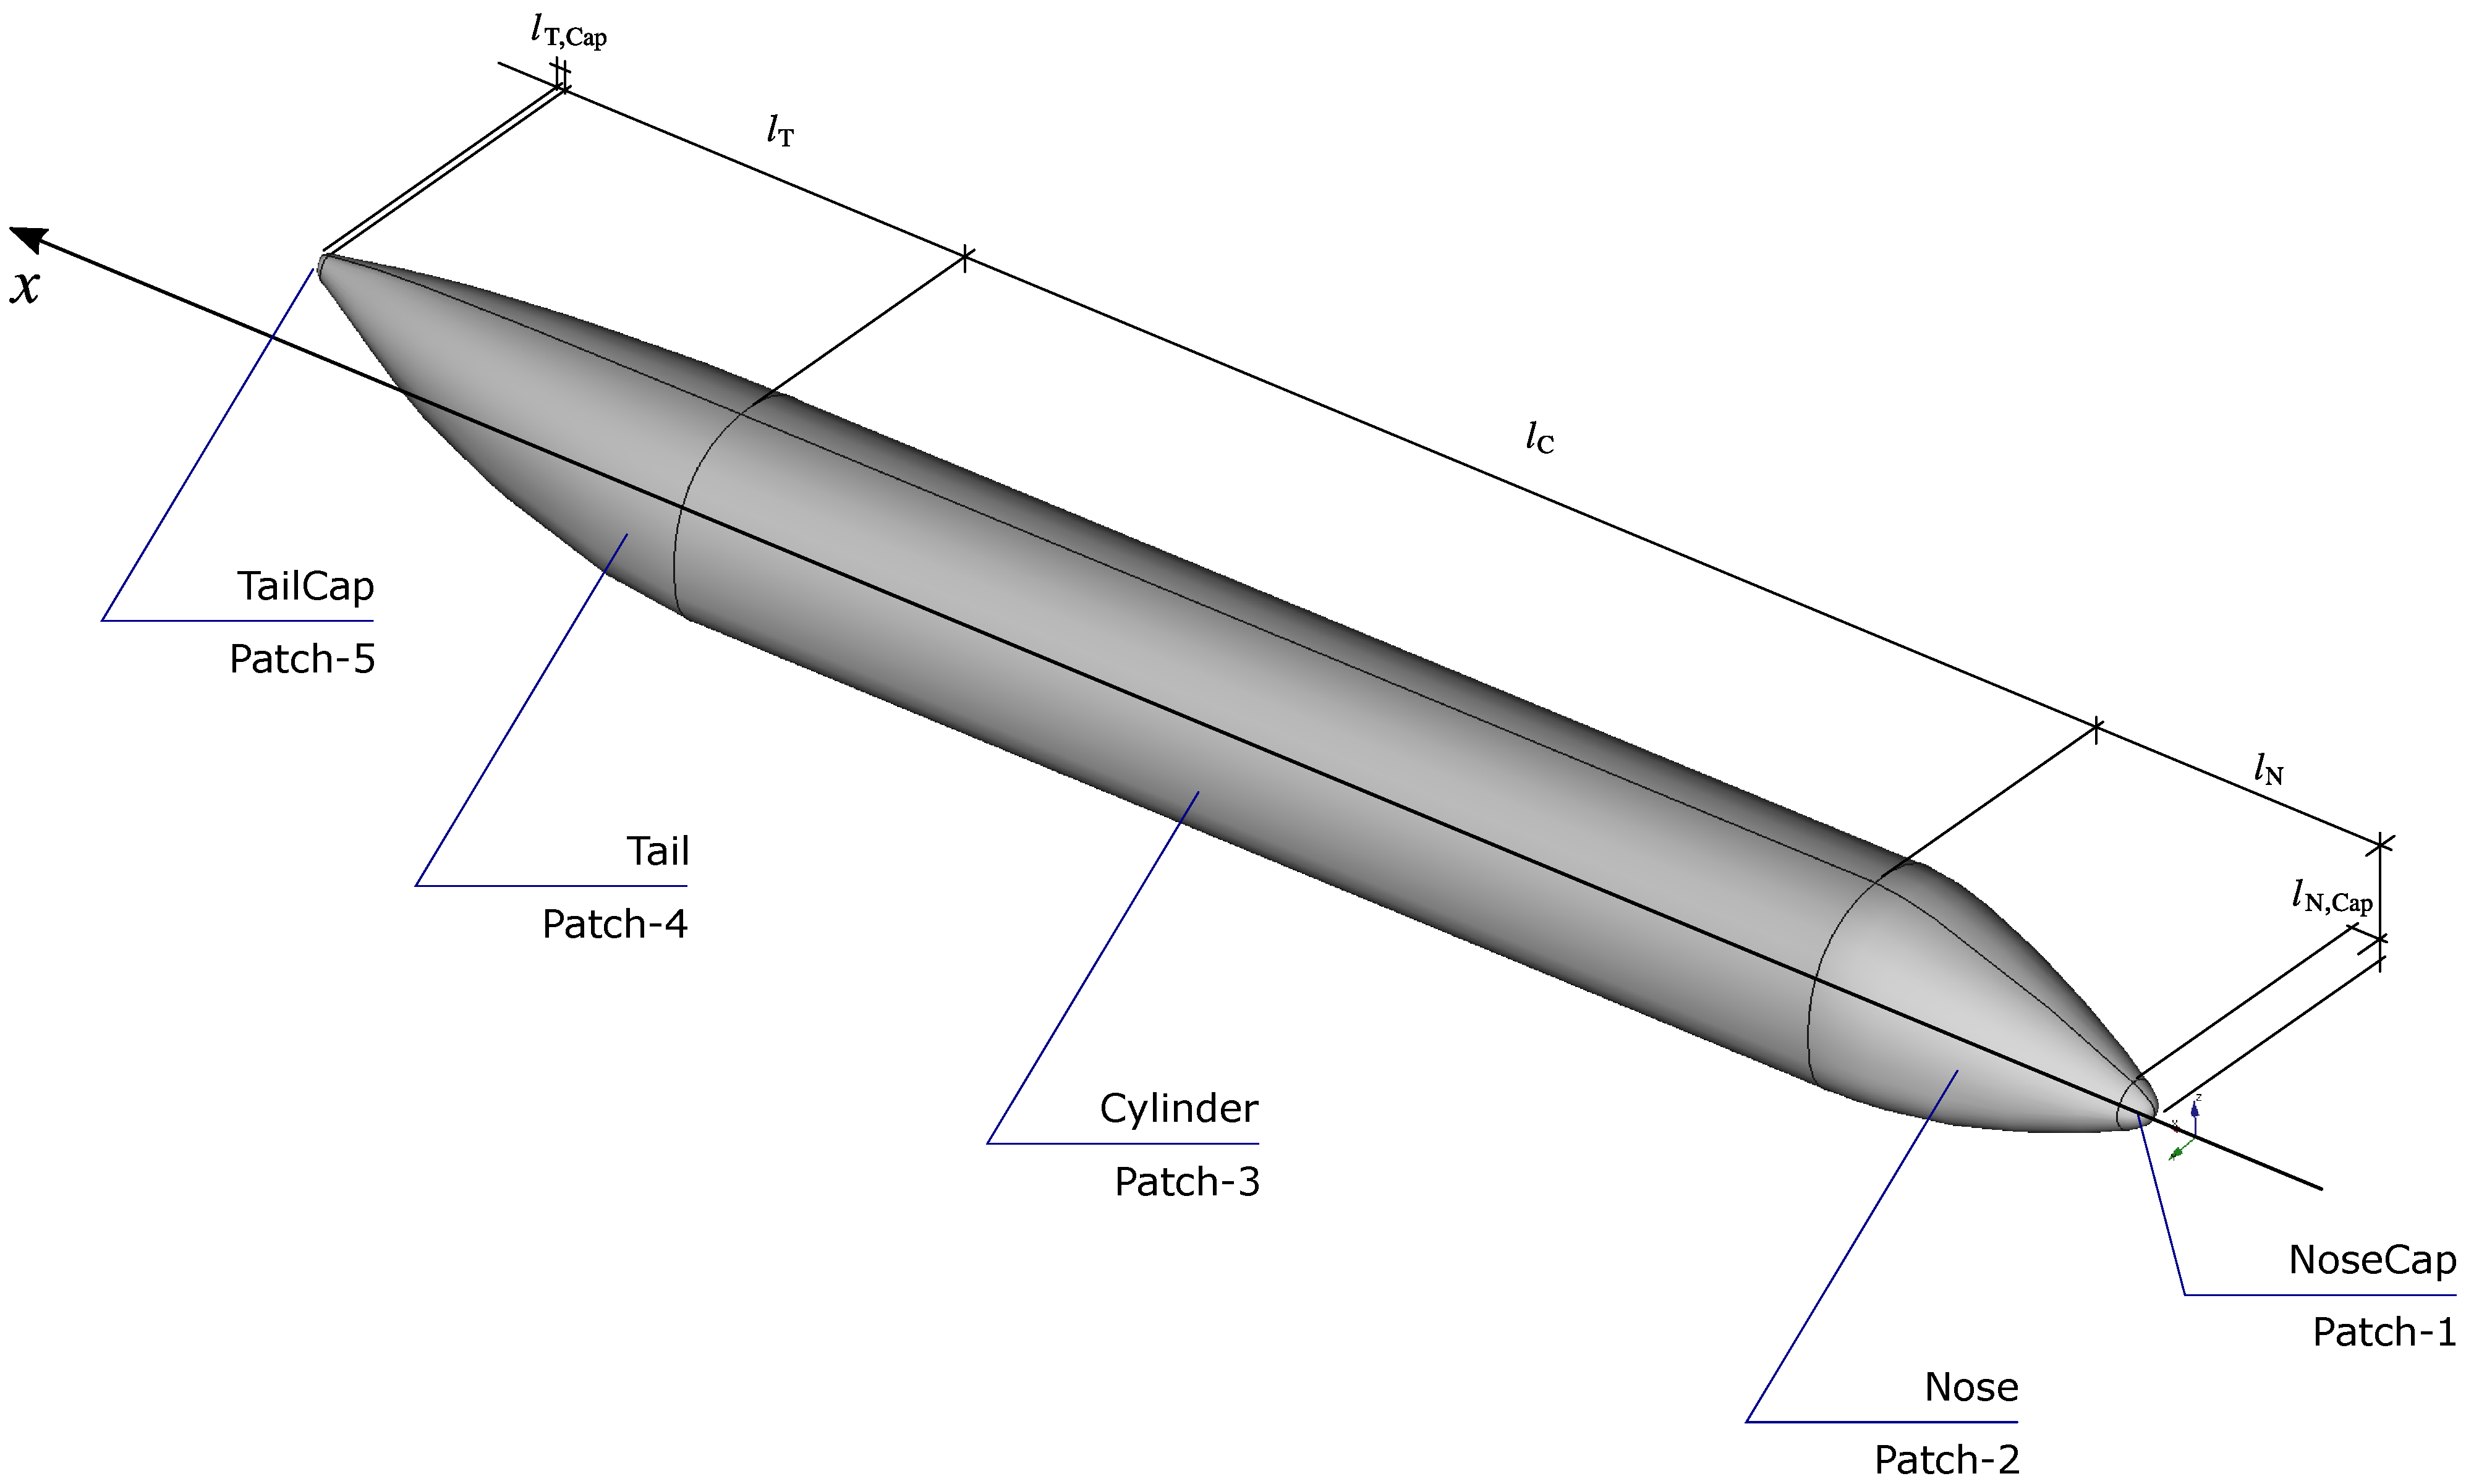
\includegraphics[scale=0.22]{Immagini/Capitolo3/fuselage_1}
\caption{Fuselage schematization for CAD purposes}
\label{fig:FusInfographic}
\end{figure}
%

\bigskip
\noindent
The algorithm can be split in two sections, with the first one providing for the generation of the lofts and the solid, while the second one is mainly dedicated to the production of the outline curves of the fuselage, completing the list of the extra shapes to be exported in case the \lstinline[language=Java]!exportSupportShapes! variable has been set to \lstinline[language=Java]!true!. After collecting essential geometric variables (such as those related to the lengths of the parts in which the fuselage has been split), the construction of the five patches that compose the fuselage begins. The building process clearly starts from the nose cap and continues till the terminal section of the fuselage.

\bigskip
\noindent
In order to determine the curves to patch through, the $x$-coordinates of the sections must be first calculated. As anticipated, the \lstinline[language=Java]!noseCapSectionFactor1! and \lstinline[language=Java]!noseCapSectionFactor2! parameters fix the position of the initial and terminal section of the nose cap patch. In particular, when respectively fixed to $0.0$ and $1.0$, first and last nose cap patch sections $x$-coordinates coincide with the actual initial and teminal $x$-coordinates of the nose cap. In order to avoid a degenerate section, the first parameter must be set to a value higher than $0.0$ (usually a value equal to $0.15$ seems to work fine). The number of nose cap sections provided to the algorithm determines how many $x$-coordinates must be calculated between initial and terminal ones, with the spacing between the sections being set to half-cosine type (with higher density towards the terminal section). \gls{JPAD} utility class \lstinline[language=Java]!MyArrayUtils! provides methods for spacing. Once all the $x$-coordinates have been determined, it is finally possible to acquire section points, by means of the \lstinline[language=Java]!Fuselage.getUniqueValuesYZSideRCurve! method. It requires the $x$-coordinates of the sections expressed in terms of \lstinline[language=Java]!Amount! (a Java class, part of the JScience package, providing support for measurements \cite{Amount}) values, and returns a list of \lstinline[language=Java]!PVector! entities, representing the coordinates of the fuselage side curve points. As the name of the method suggests, just the right curve points are returned, given the simmetry of the fuselage. For this reason, mirroring operations must be performed on lofts in order to obtain the complete shape of the fuselage, as it will be clarified in the following. Once all the lists of \lstinline[language=Java]!PVector! points have been collected, the patch for the nose cap can be finally obtained, by means of one of the \lstinline[language=Java]!OCCUtils! methods listed in Chapter \ref{chap2}. Since the patch needs to be made pass through one initial vertex and a set of curves defined by means of \lstinline[language=Java]!PVector! entities, an appropriate variant of the \lstinline[language=Java]!makePatchThruSections! methods has been used. Listing \ref{lst:NoseCapCreation} contains pieces of the actual code used to generate nose cap shapes. Variables containing the term \lstinline[language=Java]!bar! in their name hint at quantities which have been normalized with respect to the whole nose length, as specified above. 
%
\bigskip
\begin{lstlisting}[caption={Nose cap shapes building process}, captionpos=b, tabsize=2, label={lst:NoseCapCreation}]
// Determine a List containing the sections x-coordinates normalized with  
// respect to the nose length. xbarNoseCap is the normalized nose cap length. 
List<Double> xbars1 = Arrays.asList(
				MyArrayUtils
					.halfCosine2SpaceDouble(
					noseCapSectionFactor1*xbarNoseCap, noseCapSectionFactor2*xbarNoseCap, 
					numberNoseCapSections) 
				);
				

// Fill a List of PVectors for each section
List<List<PVector>> sections1 = new ArrayList<List<PVector>>();
xbars1.forEach(x -> sections1.add(
				 fuselage.getUniqueValuesYZSideRCurve(noseLength.times(x)))
	  );
	  
	
// Generate the patch for the nose cap
PVector noseTipVtx = new PVector(0.0f, 0.0f, (float) zNoseTip.doubleValue(SI.METER))	  
OCCShape patch1 = OCCUtils.makePatchThruSectionsP(
							noseTipVtx,
							sections1
							);
						
// Actually generate the supporting curves and add them to the ones to be exported
sections1.stream()
			.map(sec -> OCCUtils.theFactory
					.newCurve3D(
							sec.stream()
							.map(p -> new double[] {p.x, p.y, p.z})
							.collect(Collectors.toList()),
							false)
					)
			.map(crv -> (OCCEdge) ((OCCGeomCurve3D) crv).edge())
			.forEach(e -> extraShapes.add(e));			
\end{lstlisting}
%

\bigskip
\noindent
The patch for the nose trunk is the second to be built. The procedure is almost identical to the one previously described. The main difference consists in the fact that in this case the user is given the possibility to actually choose which kind of spacing he wants to use for the supporting curves. The \lstinline[language=Java]!spacingTypeNosePatch! variable is the one allowing this. This variable belongs to the \lstinline[language=Java]!XSpacingType! enumeration class, which will be explained in its details in the following, and being an instance of a Java \lstinline[language=Java]!enum! class it can only assume values in a close range of constant ones. Each of these constant values is associated to one of the possible spacings that can be used for a distribution of points, and each one also implements its own version of the \lstinline[language=Java]!calculateSpacing! abstract method, which belongs to the enumeration class too. The following listing contains the code used to generate the loft for the nose trunk and the supporting curves. As previously said, the variables containing the word \lstinline[language=Java]!bar! have been normalized with respect to the total length of the nose, while the ones with the word \lstinline[language=Java]!mt! (standing for \emph{meter}) are dimensional variables. Figure \ref{fig:NoseCapPlusNoseTrunk} shows the final result for the nose cap and the nose trunk shapes, highlighting the differences between the two lofts in terms of spacing and number of supporting sections.
%
\bigskip
\begin{lstlisting}[caption={Nose trunk shapes building process}, captionpos=b, tabsize=2, label={lst:NoseTrunkCreation}]
// Determine a List containing the sections x-coordinates normalized with respect 
// to the nose length. xbarNoseCap is the normalized nose cap length. 
List<Double> xbars2 = Arrays.asList(
		spacingTypePatch2.calculateSpacing(
				noseCapSectionFactor2*xbarNoseCap, 1.0,
				numberNosePatch2Sections
		));

// Generate the supporting curves for the nose 
// trunk and make them available for the export		
List<Double> xmtPatch2 = new ArrayList<>();
xbars2.forEach(x -> 
		xmtPatch2.add(x*noseLength.doubleValue(SI.METER))
		);
			  				
List<CADGeomCurve3D> cadCurvesNoseTrunk = new ArrayList<>();
xmtPatch2.stream()
		.map(x -> Amount.valueOf(x, SI.METER))
		.forEach(x -> cadCurvesNoseTrunk.add(
				OCCUtils.theFactory
						.newCurve3DP(fuselage.getUniqueValuesYZSideRCurve(x), false)
				));
					   
cadCurvesNoseTrunk.stream()
		.map(c -> (OCCGeomCurve3D) c)
		.map(crv -> (OCCEdge) (crv.edge()))
		.forEach(e -> extraShapes.add(e));

// Patch through the nose trunk supporting sections in order to obtain a loft					   
OCCShape patch2 = OCCUtils.makePatchThruSections(cadCurvesNoseTrunk);
\end{lstlisting}

\bigskip
%
\begin{figure}[H]
\centering
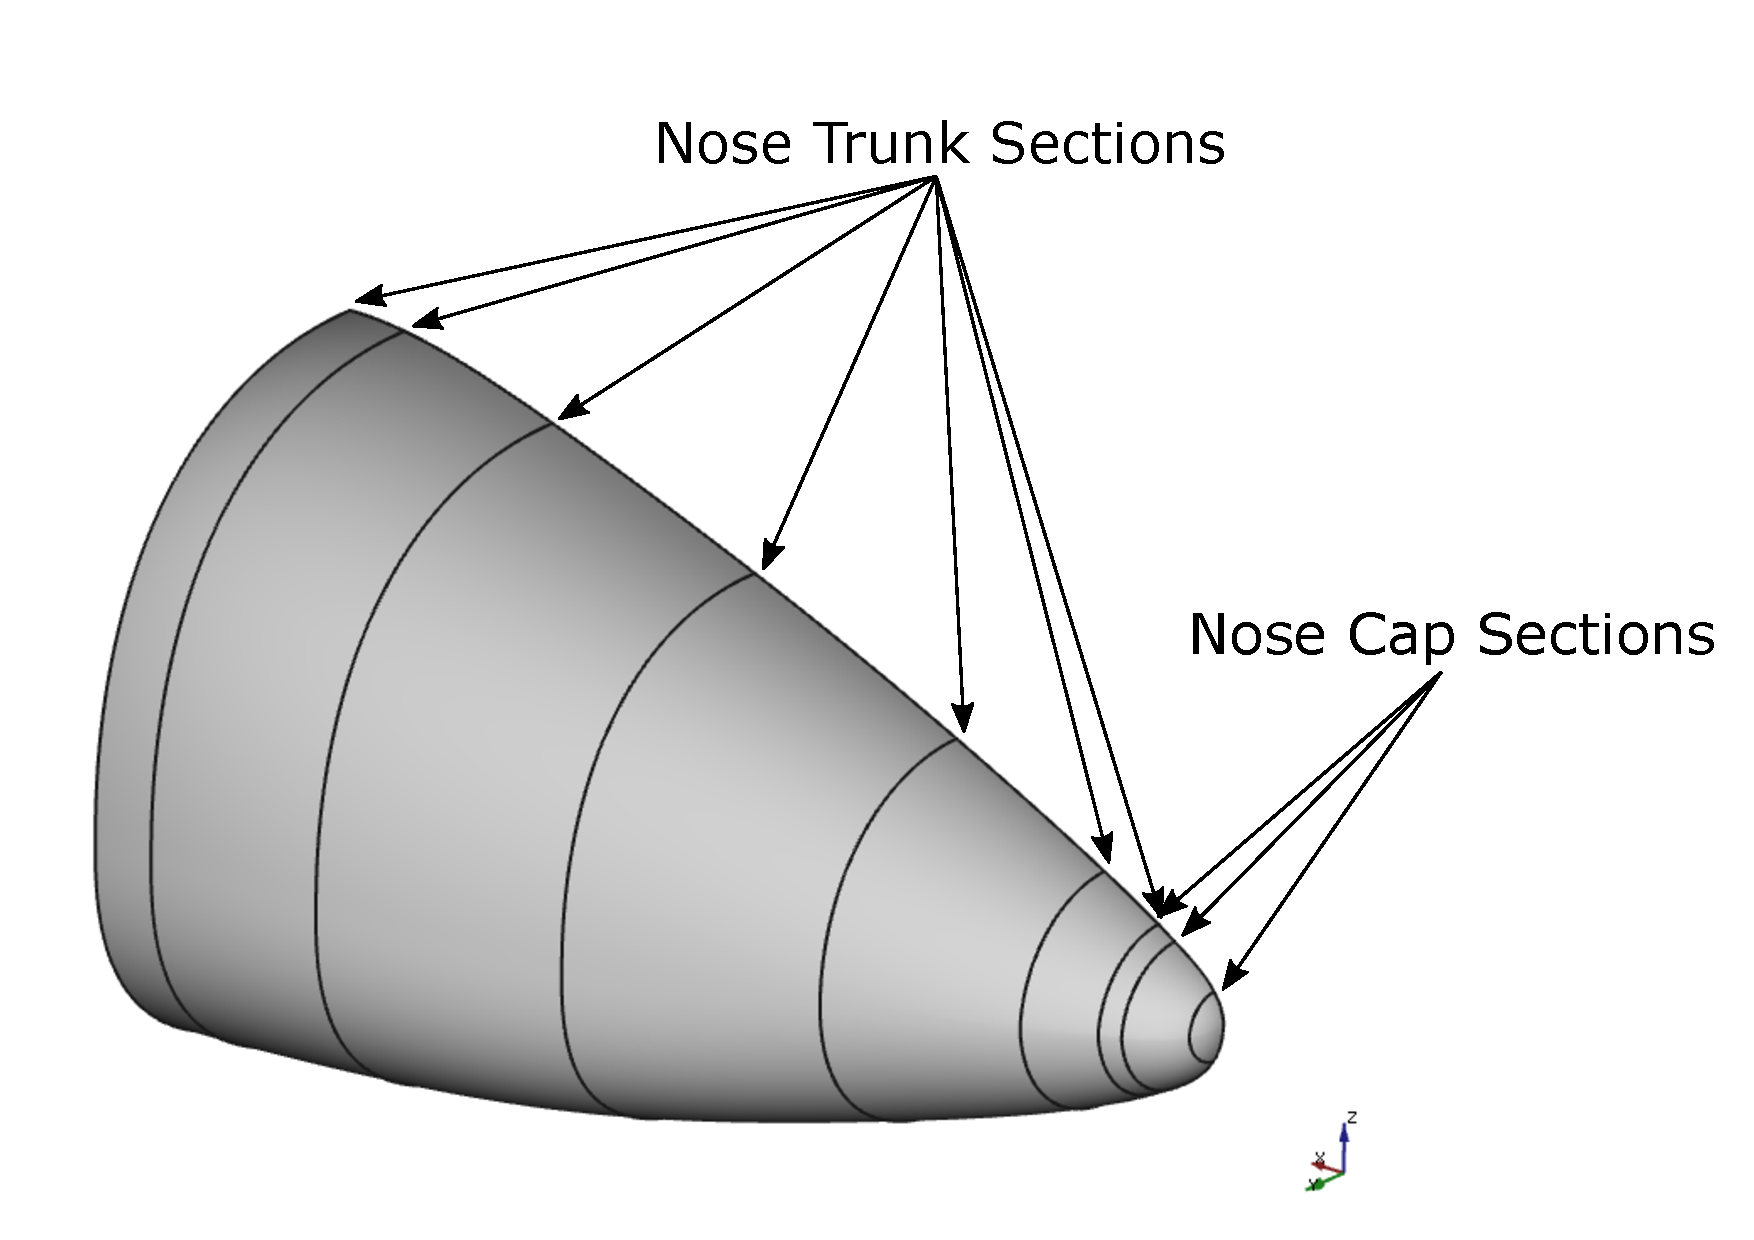
\includegraphics[scale=0.45]{Immagini/Capitolo3/nose_1}
\caption{Nose cap and nose trunk patches with supporting sections}
\label{fig:NoseCapPlusNoseTrunk}
\end{figure}
%

\bigskip
\noindent
The next step consists in generating the loft for the cylindrical section of the fuselage. This one is the easiest to obtain, since no particular attention must be paid to the number of supporting sections and the spacing between them. In fact, the \lstinline[language=Java]!getFuselageCAD! method doesn't even allow to choose the values for these parameters. Instead, the number of supporting sections is constantly set to three, with a linear spacing being used to separate them. The following lines of code describe the process through which cylindrical patch shapes have been built, with figure \ref{fig:FusCylinder} showing the result.
%
\bigskip
\begin{lstlisting}[caption={Fuselage cylinder building steps}, captionpos=b, tabsize=2, label={lst:FusCylinderCreation}]
// Determine the dimensional x-coordinates for the cylinder cross sections
List<Double> xmtPatch3 = Arrays.asList(
				MyArrayUtils.linspaceDouble(
						noseLength.doubleValue(SI.METER), 
						noseLength.plus(cylinderLength).doubleValue(SI.METER), 
						3)); // number of cross sections

// Generate supporting curves and make them available for export
List<CADGeomCurve3D> cadCrvCylinder = new ArrayList<>();
cadCrvCylinder.add(OCCUtils.theFactory.newCurve3DP(
		fuselage.getUniqueValuesYZSideRCurve(noseLength), false));				
cadCrvCylinder.add(OCCUtils.theFactory.newCurve3DP(
		fuselage.getUniqueValuesYZSideRCurve(
				noseLength.plus(cylinderLength.times(0.5))),false));				
cadCrvCylinder.add(OCCUtils.theFactory.newCurve3DP(
		fuselage.getUniqueValuesYZSideRCurve(
				noseLength.plus(cylinderLength)), false));
cadCrvCylinder.forEach(crv -> 
		extraShapes.add((OCCEdge) ((OCCGeomCurve3D) crv).edge()))	;				

// Generate the cylindrical loft by patching through the just created 3D curves.						
OCCShape patch3 = OCCUtils.makePatchThruSections(cadCrvCylinder);
\end{lstlisting}
%
\begin{figure}[H]
\centering
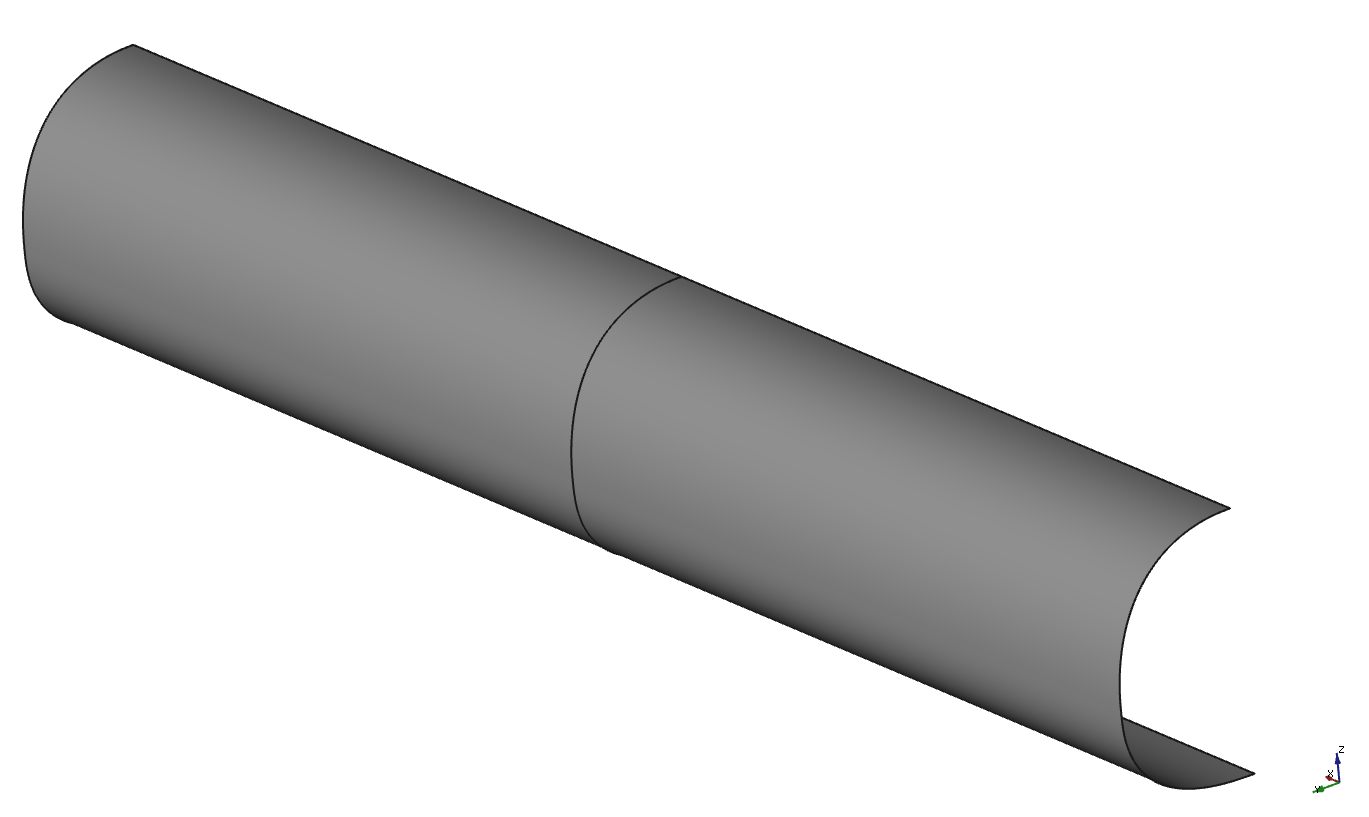
\includegraphics[scale=0.30]{Immagini/Capitolo3/FusCylinderPlusSupCurves}
\caption{Fuselage cylindrical section}
\label{fig:FusCylinder}
\end{figure}
%

\bigskip
\noindent
The generation of the tail shapes follows the same steps listed for the nose ones. The main difference consists in the different spacing adopted for the tail cap: in this case the half cosine spacing adopted forces an higher density towards the initial section of the list (so, in the negative $x$ direction). For the sake of completeness, the listing \ref{lst:TailCreation} reports part of the actual code used to generate tail shapes (including supporting sections), while figure \ref{fig:TailTrunkPlusTailCap} shows the just generated shape once being imported into a \gls{CAD} suite.
%
\bigskip
\begin{lstlisting}[caption={Tail trunk and cap building process}, captionpos=b, tabsize=2, label={lst:TailCreation}]
// Generate a list containing all tail trunk cross section x-coordinates
List<Double> xmtPatch4 = Arrays.asList(
				spacingTypeTailPatch.calculateSpacing(
						noseLength.plus(cylinderLength).doubleValue(SI.METER), 
						fuselageLength.minus(
								tailCapLength.times(tailCapSectionFactor1)).doubleValue(SI.METER), 
						numberTailPatchSections)
						);	

// Generate a list containing tail cap cross section x-coordinates				
List<Double> xmtPatch5 = Arrays.asList(
				MyArrayUtils.halfCosine1SpaceDouble(
						fuselageLength.minus(
								tailCapLength.times(tailCapSectionFactor1)).doubleValue(SI.METER), 
						fuselageLength.minus(
								tailCapLength.times(tailCapSectionFactor2)).doubleValue(SI.METER),
						numberTailCapSections) 
				);
		
// Generate tail trunk cross section curves and make them available for export.		
List<CADGeomCurve3D> cadCurvesTailTrunk = new ArrayList<>();
xmtPatch4.stream()
		.map(x -> Amount.valueOf(x, SI.METER))
		.forEach(x -> cadCurvesTailTrunk.add(
				OCCUtils.theFactory
						.newCurve3DP(fuselage.getUniqueValuesYZSideRCurve(x), false)
				));
						 
cadCurvesTailTrunk.stream()
		.map(crv -> (OCCEdge) ((OCCGeomCurve3D) crv).edge())
		.forEach(e -> extraShapes.add(e));	
		
// Generate tail cap cross section curves and make them available for export
CADVertex vertexTailTip = OCCUtils.theFactory.newVertex(
				fuselageLength.doubleValue(SI.METER), 0, zTailTip.doubleValue(SI.METER));
		
List<CADGeomCurve3D> cadCurvesTailCap = new ArrayList<>();
xmtPatch5.stream()
		.map(x -> Amount.valueOf(x, SI.METER))
		.forEach(x -> cadCurvesTailCap.add(
				OCCUtils.theFactory
						.newCurve3DP(fuselage.getUniqueValuesYZSideRCurve(x), false)
				));
						 
cadCurvesTailCap.stream()
		.map(crv -> (OCCEdge) ((OCCGeomCurve3D) crv).edge())
		.forEach(e -> extraShapes.add(e));	
		
// Generate the patch for the tail trunk
OCCShape patch4 = OCCUtils.makePatchThruSections(cadCurvesTailTrunk);


// Generate the patch for the tail cap
OCCShape patch5 = OCCUtils.makePatchThruSections(
		cadCurvesTailCapTrunk, vertexTailTip);
\end{lstlisting}
%

\bigskip
%
\begin{figure}[H]
\centering
\includegraphics[scale=0.40]{Immagini/Capitolo3/tail_1}
\caption{Tail cap and tail trunk patches with supporting sections}
\label{fig:TailTrunkPlusTailCap}
\end{figure}
%

\bigskip
\noindent
Once all the lofts have been created, they need to be sewed, in order to get one single shell. The \gls{OCCT} library provides the class to perform this kind of operation: it is called \lstinline[language=Java]!BRepBuilderAPI_Sewing! and provides methods in order to:
%
\begin{itemize}
\item create an empty builder,
\item add elements (generic shapes) to the builder,
\item set the tolerance,
\item compute the operation,
\item return the resulted shapes. 
\end{itemize}
%
The \lstinline[language=Java]!CADShapeFactory! actually contains methods in order to perform sewing operations, but starting from \lstinline[language=Java]!CADFace! instances. Since the shape we need to sew are actually shells, and sewing methods managing shell-type elements still need to be implemented in \lstinline[language=Java]!JPADCAD!, the actual code makes direct use of the \gls{OCCT} class. This is not the only case (as it will be clear in the next paragraphs and chapters), since \lstinline[language=Java]!JPADCAD! is still under constant development and testing. 
%
\bigskip
\begin{lstlisting}[caption={Lofts sewing process}, captionpos=b, tabsize=2, label={lst:PatchSewing}]
// Generate a new instance of the sewmaker class
BRepBuilderAPI_Sewing sewMaker = new BRepBuilderAPI_Sewing();

// Initalize the sewmaker and provide it with the patches.
// Finally, perform the sewing operation. 
sewMaker.Init();
sewMaker.Add(patch1.getShape());
sewMaker.Add(patch2.getShape());
sewMaker.Add(patch3.getShape());
sewMaker.Add(patch4.getShape());
sewMaker.Add(patch5.getShape());
sewMaker.Perform();

// Get the resulting TopoDS_Shape entity
TopoDS_Shape tds_shape = sewMaker.SewedShape();
\end{lstlisting}

\bigskip
\noindent
Once the sewing operation has been performed, the returned shape must be explored, in order to find shell-type entities. This operation is performed by means of the \lstinline[language=Java]!CADShapeFactory! method \lstinline[language=Java]!newExplorer!, which relies on the \lstinline[language=Java]!OCCExplorer! class constructors and allows to generate some sort of \emph{seeker} for desired shapes. This operation is fundamental, since the shape returned by the sewing algorithm belongs to the abstract \gls{OCCT} \lstinline[language=Java]!TopoDS_Shape! class.

\bigskip
\noindent
The next operation consists in mirroring the fuselage right shell obtained at the previous step. As mentioned in Chapter \ref{chap2}, the \gls{OCCT} library offers the possibility to perform basic geometry transformations. The class supervising this type of operation is called \lstinline[language=Java]!gp_Trsf!, which actually allows to perform:
%
\begin{itemize}
\item translation,
\item rotation,
\item scale,
\item reflection with respect to a point, a line, a plane.
\end{itemize}
%
The type of the operation can be choosed by means of several \lstinline[language=Java]!set! methods, that act directly on an empty instance of the \lstinline[language=Java]!gp_Trsf! class. In our case, a plane (the plane of symmetry of the fuselage) must be defined in order to perform the mirroring operation. The \gls{OCCT} class \lstinline[language=Java]!gp_Ax2! helps defining a plane by means of a point (the origin, expressed in terms of \lstinline[language=Java]!gp_Pnt!), and two directions (both expressend in terms of instances of the \gls{OCCT} class \lstinline[language=Java]!gp_Dir!), identifying the normal to the plane and a direction contained in the same plane. The following listing shows how the operation has been coded.
%
\bigskip
\begin{lstlisting}[caption={Fuselage right shell mirroring operations}, captionpos=b, tabsize=2, label={lst:ShellMirroring}]
// Define a new instance of the transformation class
gp_Trsf mirrorTransform = new gp_Trsf();

// Define the plane with respect to the shapes must be mirrored
gp_Ax2 mirrorPointPlane = new gp_Ax2(
		new gp_Pnt(0.0, 0.0, 0.0), // Origin
		new gp_Dir(0.0, 1.0, 0.0), // Y direction
		new gp_Dir(1.0, 0.0, 0.0)  // X direction
		);

// Select the the transformation to perform, add to it the just 
// created plane and generate a new instance of the actual OCCT
// class executing transformation on shape geometries
mirrorTransform.SetMirror(mirrorPointPlane);
BRepBuilderAPI_Transform mirrorBuilder = 
		new BRepBuilderAPI_Transform(mirrorTransform);
		
// Finally perform the mirroring operation
mirrorBuilder.Perform(sewedShell.getShape(), 1);
TopoDS_Shape mirroredShape = mirrorBuilder.Shape();
\end{lstlisting}

\bigskip
\noindent
In this case too it is necessary to go through the shapes produced by the mirroring operations in order to find shell-type entities. The operation performed is the same described above. Once the shells for the right and left side of the fuselage have been obtained, another sewing operation can be executed, returning one single shell, which will be the one to be used in order to create a solid entity. Altough the \lstinline[language=Java]!CADShapeFactory! contains methods generating solids, the ones currently implemented do not allow the production starting from shells. For this reason, at present, the code performs the creation of solid entities by using low level \gls{OCCT} classes. In particular, the class that implements this type of operation is called \lstinline[language=Java]!BRepBuilderAPI_MakeSolid! which provides methods for:
%
\begin{itemize}
\item defining and implementing the construction of a solid,
\item consulting the results.
\end{itemize}
%
Once the shell has been added to an empty instance of the solid builder class, the user just needs to use the \lstinline[language=Java]!Build! method in order to perform the construction. Figure \ref{fig:FusSolid} shows different views of the same solid fuselage, with the one depicted belonging to the ATR-72. 
%
\bigskip
\begin{lstlisting}[caption={Fuselage solid building step}, captionpos=b, tabsize=2, label={lst:FuselageSolid}]
// Generate a CADSolid empty instance 
CADSolid solidFuselage = null;

// Generate a new solidmaker empty object
BRepBuilderAPI_MakeSolid solidMaker = new BRepBuilderAPI_MakeSolid();

// Add the sewed halves of the fuselage to the solidmaker
// and perform the building operation
solidMaker.Add(TopoDS.ToShell(sewedShells.getShape()));
solidMaker.Build();

// Finally generate the fuselage CADSolid object by means of the
// OCCUtils newShape method, which accept a generic object of 
// the underlying implementation to build CAD-type ones
if(solidMaker.IsDone() == 1) {
		solidFuselage = (CADSolid) OCCUtils.theFactory.newShape(solidMaker.Solid());
}
\end{lstlisting}

\bigskip
\noindent
The \lstinline[language=Java]!getFuselageCAD! method implemented in \lstinline[language=Java]!AircraftUtils! allows not only to export the final solid shape of the fuselage. It also gives the user the possibility to choose between which types of shape he wants to export and write to file. For example, by setting to \lstinline[language=Java]!true! the \lstinline[language=Java]!exportSupportShapes! parameter and \lstinline[language=Java]!false! the remaining ones, just the wireframe of the fuselage would be exported. For sake of completeness, figure \ref{fig:FusWireframe} shows the wireframe (completed by the outline curves, whose calculation is performed by the code but not actually used for loft generation purposes) of the fuselage of the ATR-72.

\bigskip
%
\begin{figure}[H]
\centering
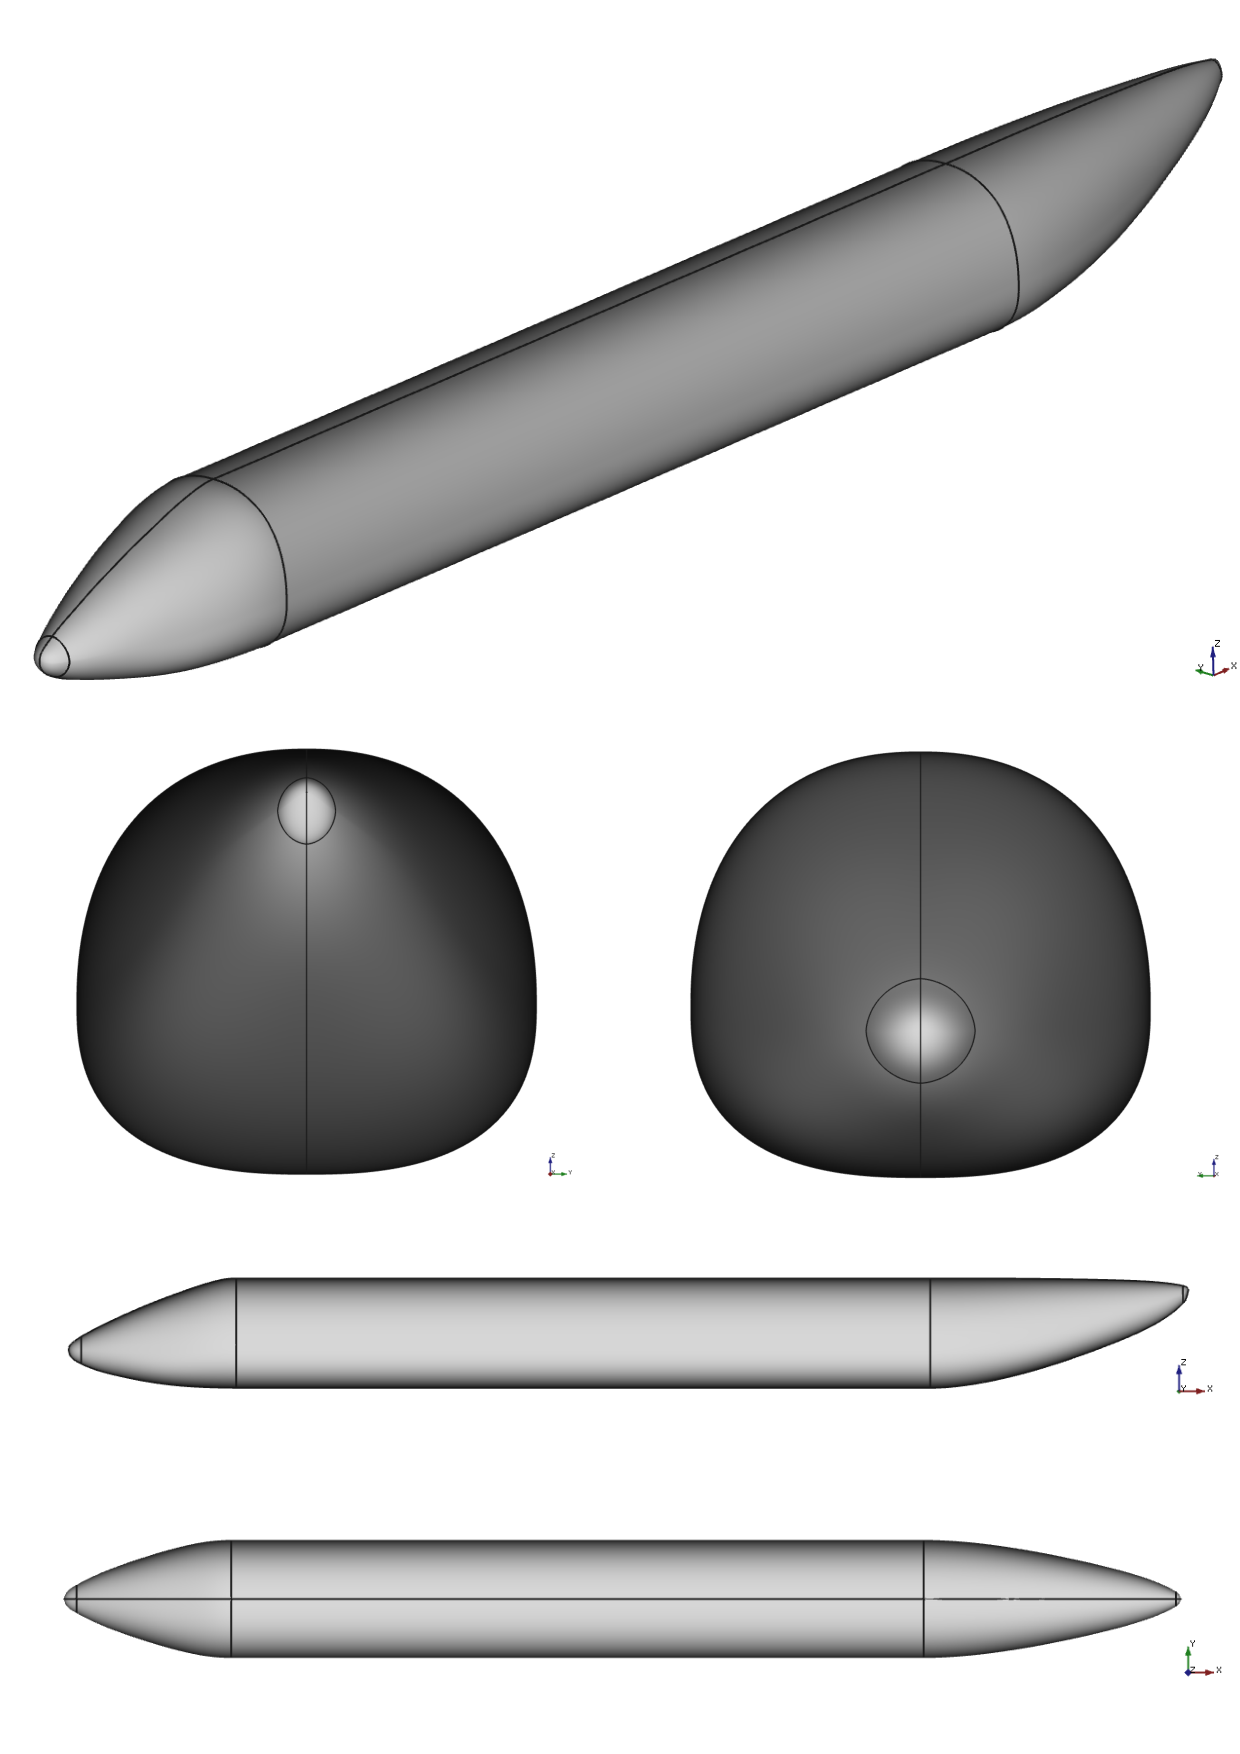
\includegraphics[scale=0.45]{Immagini/Capitolo3/fussolid_1}
\caption{ATR-72 solid fuselage, different views}
\label{fig:FusSolid}
\end{figure}
%
\begin{figure}[H]
\centering
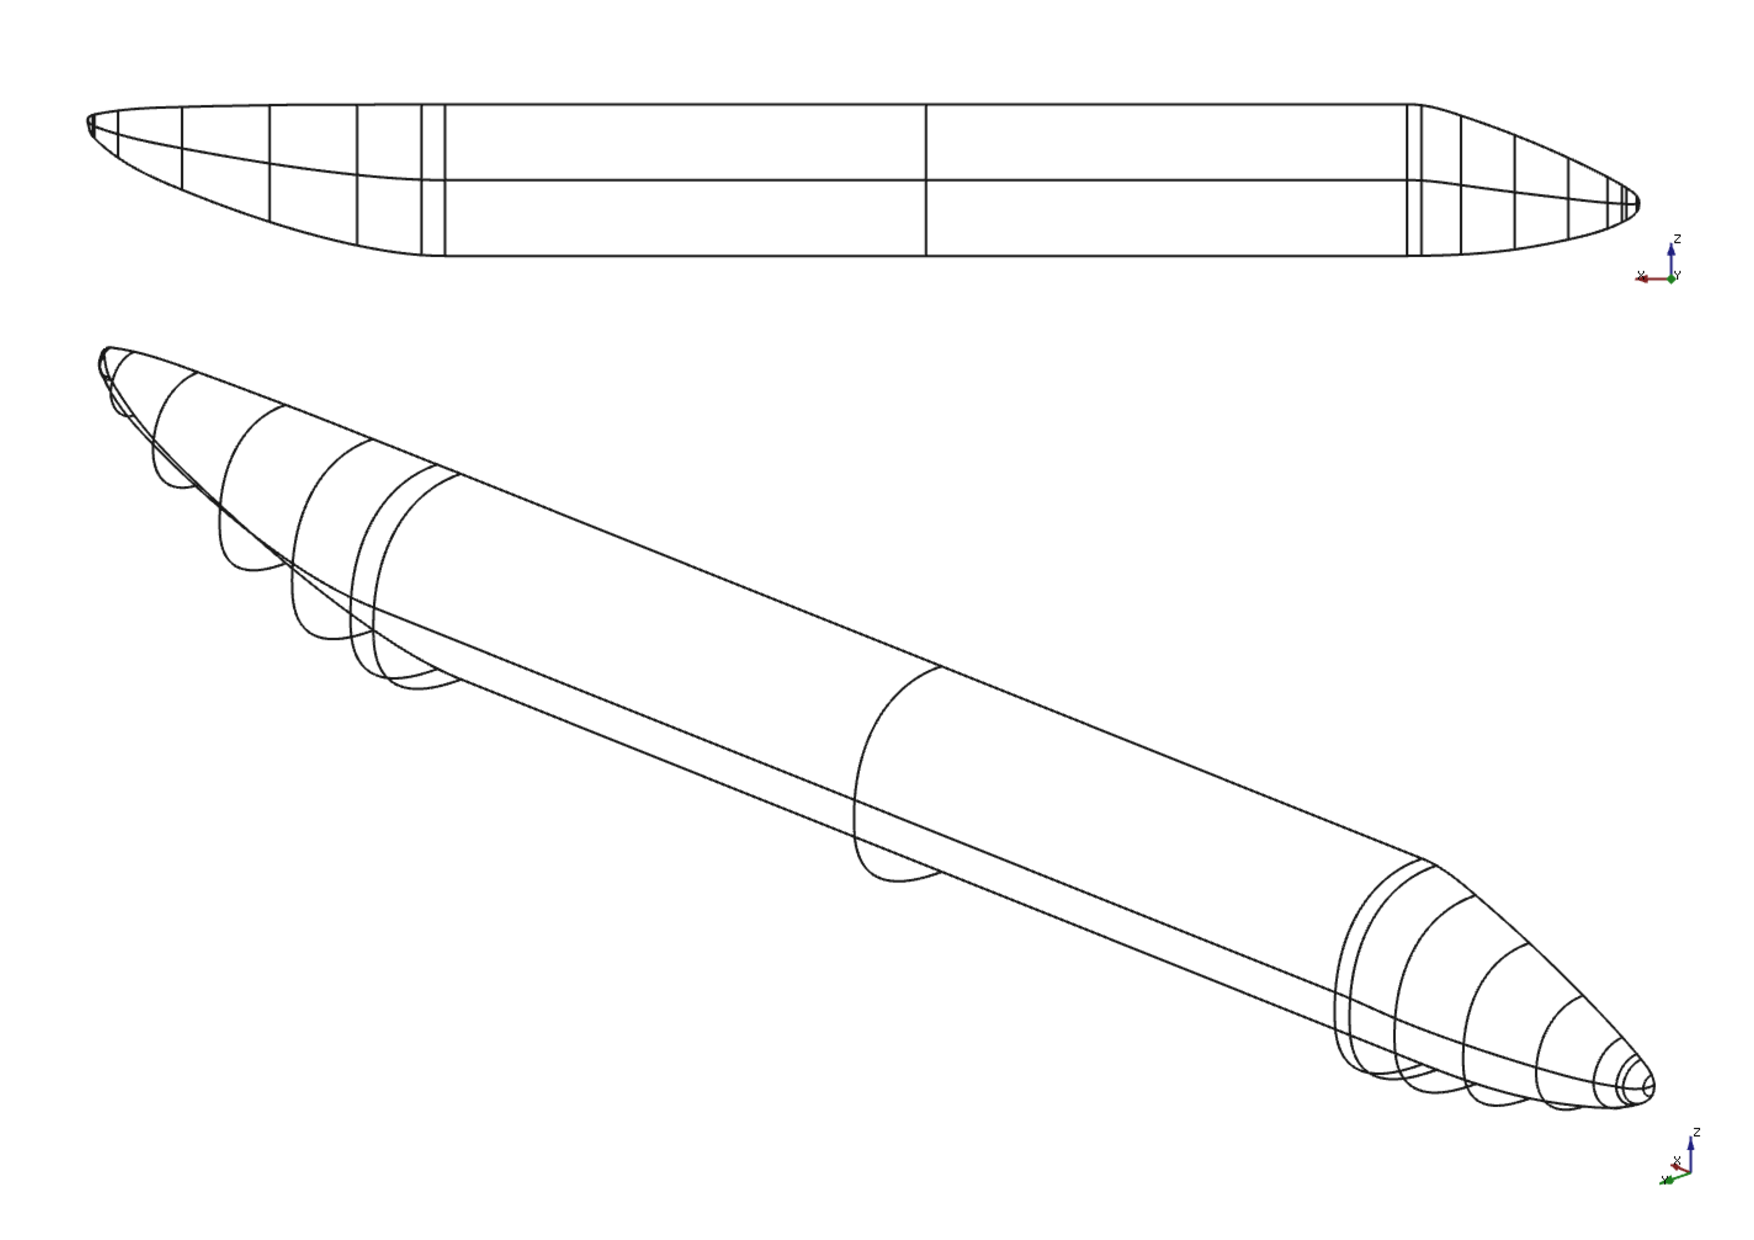
\includegraphics[scale=0.32]{Immagini/Capitolo3/fuswireframe_1}
\caption{ATR-72 fuselage wireframe, different views}
\label{fig:FusWireframe}
\end{figure}

\section{Lifting surface CAD method}
\label{sec3.4}

The construction of the shapes representing a generic lifting surface revolves around three main stages, tipically:
%
\begin{enumerate}
\item generate one loft for each panel of the wing;
\item generate a shell for the tip of the wing;
\item reflect the resulting shapes with respect to a symmetry plane (whether necessary).
\end{enumerate}
%
\begin{figure}[H]
\centering
\includegraphics[scale=0.47]{Immagini/Capitolo3/wing_1}
\caption{Wing patches for a JPAD wing}
\label{fig:WingPatches}
\end{figure}
%
The \lstinline[language=Java]!AircraftUtils! method that provides for the construction of lifting surfaces is called \lstinline[language=Java]!getLiftingSurfaceCAD!. This method accepts the following inputs.
%
\begin{itemize} 
\renewcommand\labelitemi{\tiny$\blacksquare$}
\renewcommand\labelitemii{\tiny$\bullet$}
\item \textbf{\lstinline[language=Java]!liftingSurface!} - An instance of the JPAD \lstinline[language=Java]!LiftingSurface! class, that is used in order to describe and collect geometric, aerodynamic and mass characteristics of a generic lifting surface. It provides also the methods to access all these information.
\item \textbf{\lstinline[language=Java]!typeLS!} - An instance of the JPAD \lstinline[language=Java]!ComponentEnum! class, which provides support for aircraft components enumeration. The \lstinline[language=Java]!getLiftingSurfaceCAD! algorithm makes use of this argument in order to distinguish between different typologies of lifting surfaces. It is necessary for the code to know with which kind of surface it is dealing with, in order to perform the necessary checks and to activate the right flags for certain types of operations.
\item \textbf{\lstinline[language=Java]!tipTolerance!} - A \lstinline[language=Java]!double! entry fixing the tolerance for the process of sewing the tip of the lifting surface (which is modeled separately) with the rest of the wing.
\item \textbf{\lstinline[language=Java]!exportLofts!, \lstinline[language=Java]!exportSolid!, \lstinline[language=Java]!exportSupportShapes!} - Entries of the \lstinline[language=Java]!boolean! type, that allow to export, respectively, the shells (wing and tip), the solid, and the wireframe of the lifting surface.
\end{itemize}
%
\noindent
First things the algorithm executes regard data collection (by means of the methods provided by the \lstinline[language=Java]!LiftingSurface! class) and the wing wireframe construction. One of the datum that must be collected is the one related to the number of panels that constitute the wing. This number is tipically equal to two for proper wings, one for the other lifting surfaces such as the tail ones and the canard. Once all the necessary data has been collected, the construction of the wireframe of the wing can begin. For this purpose, leading edge, trailing edge, and airfoil curves must be created. It has to be noted that, as for the fuselage construction, some of the wireframe shapes generated are not intended to be used for lofting operations. Leading and trailing edge segments, for example, just serve for graphical purposes, and are not actually used as guide curves when performing patching. Furthermore, being generated by means of just two points (obtained by wing breakpoints coordinates), these edges are just segments and do not follow the actual profile of the curves they are meant to represent. On the contrary, airfoil curves are actually used to generate lofts, by patching through them using the same algorithms described in the previous paragraph and in Chapter \ref{chap2}. The \lstinline[language=Java]!liftingSurface! object passed to the method allows access to the list of airfoils located at the wing breakpoints. This list contains objects of the \lstinline[language=Java]!Airfoil! type, which is the class that in \gls{JPAD} manages aerodynamic and geometric characteristics of airfoils, and provides methods that give access to the $x$ and $z$ coordinates of its points. Since these points just define the \emph{absolute} airfoil (the airfoil with its chord aligned with the $x$ axis and length equal to $1$), they need to be modified in order to correctly represent the actual airfoils at some precise locations along the lifting surface. The \lstinline[language=Java]!AircraftUtils! class has then been provided with a private method called \lstinline[language=Java]!populateCoordinateList!. This method receives:
%
\begin{itemize}
\item a \lstinline[language=Java]!double! representing the $y$ station at which the airfoil points must be calculated;
\item an object of the \lstinline[language=Java]!Airfoil! class, which provides the basic airfoil points;
\item an object of the \lstinline[language=Java]!LiftingSurface! type, that provides wing characteristics (in terms of chord length, twist angle, and leading edge coordinates) at precise locations along its span;
\end{itemize}
and returns a \gls{List} of \lstinline[language=Java]!double[]! points, representing the actual coordinates of the airfoil. This method also performs several checks on the points it is supplied to. A first check is made on the points imported from the \lstinline[language=Java]!Airfoil! object by controling there are no duplicates among the list, in order to avoid problems once the spline interpolation needs to be performed. Another check is made on the trailing edge of the airfoil, which has to be opened in case the $z$ coordinates of the first and last points of the list coincide. This is a necessary operation, especially when the import of the \gls{CAD} model of the wing into a \gls{CFD} suite is something planned. Currently the method does not allow to adjust the value of the gap between the points: the code automatically opens the trailing edge if the distance between the first and the last point of the basic airfoil is less than $10^{-5}\si{\meter}$ in the $z$ direction, setting it to $10^{-4}\si{\meter}$.
%
\bigskip
\begin{lstlisting}[caption={Opening creation at the trailing edge}, captionpos=b, tabsize=2, label={lst:OpeningTE}]
if(Math.abs(zCoords[0] - zCoords[nPoints - 1]) < 1e-5) {
			zCoords[0] += 5e-4;
			zCoords[nPoints - 1] -= 5e-4;
		}
\end{lstlisting}

\bigskip
\noindent
Once the points have been obtained, they can be interpolated by means of one of the factory methods for 3D curves seen in Chapter \ref{chap2}. These methods interpolate a list of points by using a \gls{acr:NURBS} curve and provide a \lstinline[language=Java]!CADGeomCurve3D! object representing the curve itself. Figure \ref{fig:AirfoilSample} shows an example of an airfoil obtained by applying the aforementioned methods. In particular, the figure depicts a NACA 23018 airfoil.
%
\begin{figure}[H]
\centering
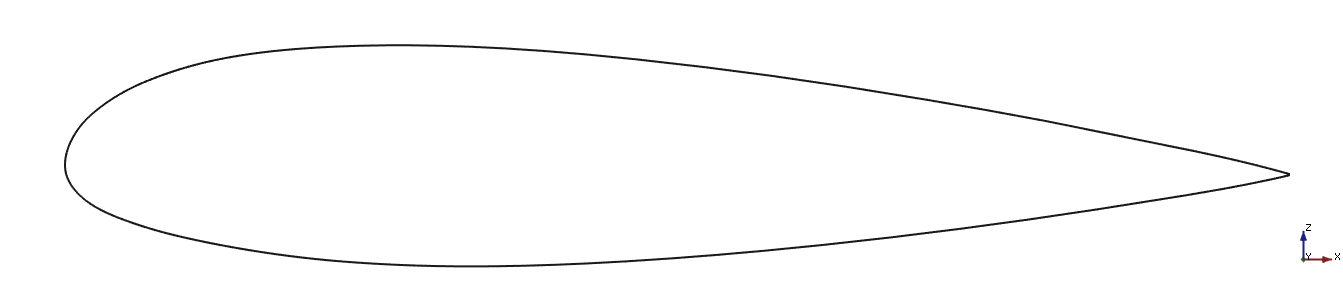
\includegraphics[scale=0.28]{Immagini/Capitolo3/WingAirfoil}
\caption{NACA 23018 airfoil curve generated in JPAD}
\label{fig:AirfoilSample}
\end{figure}
%
\noindent
The method described above allows to build airfoils at every desired location along the wing span. A first group of airfoils is generated at the breakpoints, while secondary groups are created between them. The reason behind having multiple airfoils between breakpoint ones resides in the necessity to create wing lofts, one for each panel, by patching through more than just two airfoil curves at a time, in order to reduce the risk of having unexpected results and to increase final shapes adherence to real counterparts. Since the number of panels is not something that can be known \emph{a priori} when applying \gls{CAD} generating methods for lifting surfaces, the user is not currently enabled to fix the number of cross sections for each patch. However, the code automatically sets it, based on the length of each panel respet to the total wing span. At the end of this process, a list of lists of \lstinline[language=Java]!CADGeomCurve3D! is filled, with each of the sub-lists associated to a specific panel. Figure \ref{fig:WingWireframe} shows the wireframe created to this point, with breakpoints airfoils also provided with their chord segment.
%
\begin{figure}[H]
\centering
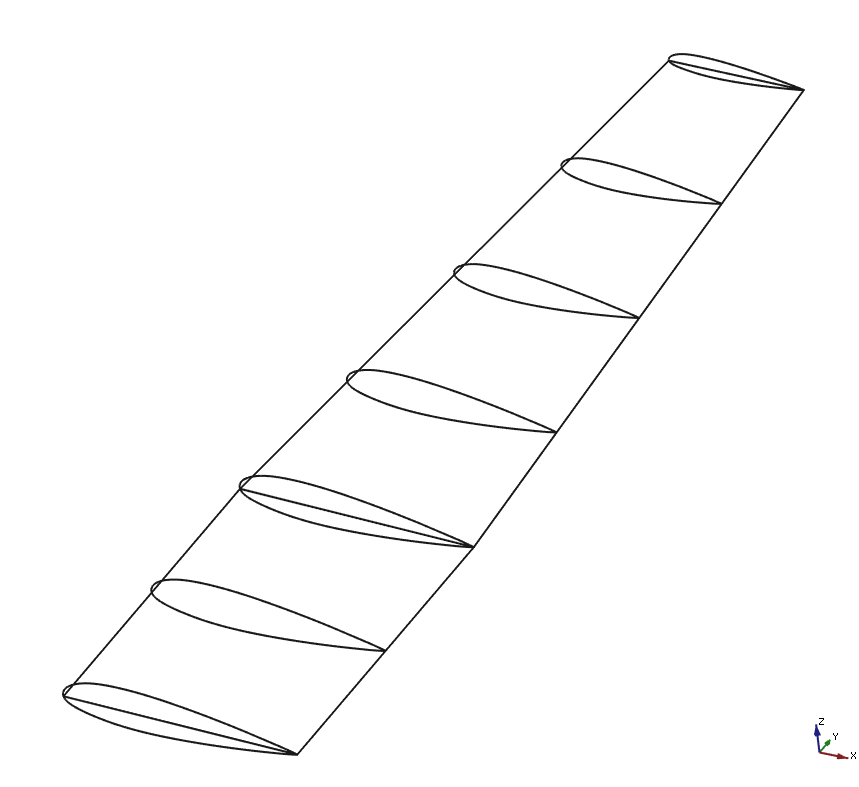
\includegraphics[scale=0.42]{Immagini/Capitolo3/WingWireframe}
\caption{Wing wireframe, with no sketching curves for the tip}
\label{fig:WingWireframe}
\end{figure}
% 

\bigskip
\noindent
As mentioned before, the \lstinline[language=Java]!getLiftingSurfaceCAD! method also generates shapes for the wing tip. These shapes are created by following the same steps used for the construction of fuselage and wing patches. The main difference in this case consists in the fact that the curves to patch through needs to be created from scratch, since \gls{JPAD} \lstinline[language=Java]!LiftingSurface! class does not contain a description for the tip. The very first operation consists in splitting the tip and penultimate airfoils (i.e., the last and the second-to-last of the airfoils depicted in figure \ref{fig:WingWireframe}) in two halves at their leading edge, by means of the wing wireframe generated at the previous step. These operations are necessary for two reasons:
%
\begin{itemize}
\item allow to better shape the leading edge of the wing tip by splitting its filling process in two steps, one regarding the upper side and one regarding the lower one;
\item the algorithm that has been implemented in order to generate the cross sections for the wing tip necessitates both the upper and the lower side curves of the tip and pre-tip (penultimate) airfoils. 
\end{itemize}
%
Besides, since it is quite likely that the leading edge of the tip airfoil does not precisely pass through the points of the leading edge of the wing wireframe, a further manipulation is necessary. This operation consists in forcing the two halves of the tip airfoil to pass through the last of the points describing the leading edge wireframe, and, in order to make sure the two halves preserve their original shape as much as possible, a much larger number of points is used to discretize them. This operation is quite necessary, since in case the condition described above is not satisfied the filling operations for the wing tip leading edge could encounter some problematics while are executed. 

\bigskip
\noindent
In order to build the necessary supporting curves for the tip shell, some construction must be performed first. For one thing, some sort of supporting plane is built, by simply extending the leading and trailing edge segments of the wing wireframe in the positive $y$ direction. The amount of this extension is related to the thickness of the tip airfoil. This extension generates the points A and B (figure \ref{fig:WingTip1}), and the segments a, b, and c, that define the actual construction plane for the wing tip. These operations are performed by means of \lstinline[language=Java]!PVector! objects, that prove to be really useful especially when managing directions and point definitions. In order to obtain an authentic plane at the previous step, point B $z$ coordinate is slightly changed and adjusted (whether the lifting surface being built is not a vertical tail) in order to make it coincide with the one of point A. Once the construction plane has been obtained, it is possible to build the first of the supporting curves for the tip. The points for this curve are obtained by using the \lstinline[language=Java]!PVector! class too, which provides static methods to perform linear interpolation between one vector and another. In particular, the point C is the point at the $25\%$ of the segment b (that has been oriented from A to B, so in the positive $x$ direction), while the point D is at the $75\%$ of the same segment. Point E is at the $75\%$ of the segment connecting the leading and trailing edge of the tip airfoil, while F is at the $90\%$ of the edge that connects the points D and E. Finally, point G is obtained as the point at the $25\%$ of the segment c. 
%
\bigskip
\begin{lstlisting}[caption={Points for the in-plane tip construction curve}, captionpos=b, tabsize=2, label={lst:ConstCurvePnts}]
double[] mainVSecVector = {0.25, 0.75};
PVector cPnt = PVector.lerp(aPnt, bPnt, (float) mainVSecVector[0]);
PVector dPnt = PVector.lerp(aPnt, bPnt, (float) mainVSecVector[1]);	
PVector ePnt = PVector.lerp(le2, te2, (float) mainVSecVector[1]);
PVector fPnt = PVector.lerp(ePnt, dPnt, 0.90f);	
PVector gPnt = PVector.lerp(bPnt, te2, 0.25f);
\end{lstlisting}

\bigskip
\noindent
In order to shape the in-plane construction curve correctly, tangent vectors must be assigned. In particular, the curve is assigned three tangency constraints: one in A, one in C, and the last one in G. These tangent vectors are obtained by means of several \lstinline[language=Java]!PVector! entities manipulations. Since the \gls{OCCT} algorithm underlying the \lstinline[language=Java]!newCurve3D! factory methods allow to assign tangency constraints only at the initial and final points of a curve, two in-plane construction curves are actually built, with the second one being split (at the point F) by means of the \lstinline[language=Java]!OCCUtils.splitEdge! method, in order to facilitate the subsequent necessary manipulations (listing \ref{lst:ConstrCurves}).
%
\bigskip
\begin{lstlisting}[caption={In-plane construction curves building steps}, captionpos=b, tabsize=2, label={lst:ConstrCurves}]
// Point lists for the in-plane construction curves
List<double[]> constrPlaneGuideCrv1Pnts = new ArrayList<>();
constrPlaneGuideCrv1Pnts.add(new double[] {le2.x, le2.y, le2.z});
constrPlaneGuideCrv1Pnts.add(new double[] {cPnt.x, cPnt.y, cPnt.z});
		
List<double[]> constrPlaneGuideCrv2Pnts = new ArrayList<>();
constrPlaneGuideCrv2Pnts.add(new double[] {cPnt.x, cPnt.y, cPnt.z});
constrPlaneGuideCrv2Pnts.add(new double[] {fPnt.x, fPnt.y, fPnt.z});
constrPlaneGuideCrv2Pnts.add(new double[] {gPnt.x, gPnt.y, gPnt.z});

// Generate tangent vectors
PVector leVector = PVector.sub(le2, le1); // Vector representing the LE segment
PVector aVector = PVector.mult(leVector, aLength);
PVector cVector = PVector.sub(cPnt, aPnt); 
PVector gVector = PVector.sub(gPnt, fPnt);

// Weights for the tangency constraints
double tanAFac = 1;
double tanCFac = (cVector.mag()/aVector.mag())*0.75;
double tanGFac = tanCFac;

// Tangent vectors normalization
aVector.normalize();
cVector.normalize();
gVector.normalize();	
		
// Actual tangent vectors for the construction curves.
double[] tanAConstrPlaneGuideCrv = MyArrayUtils.scaleArray(
		new double[] {aVector.x, aVector.y, aVector.z}, tanAFac);
double[] tanCConstrPlaneGuideCrv = MyArrayUtils.scaleArray(
		new double[] {cVector.x, cVector.y, cVector.z}, tanCFac);
double[] tanGConstrPlaneGuideCrv = MyArrayUtils.scaleArray(
		new double[] {gVector.x, gVector.y, gVector.z}, tanGFac);

// Points interpolation
CADGeomCurve3D constrPlaneGuideCrv1 = OCCUtils.theFactory.newCurve3D(
				constrPlaneGuideCrv1Pnts, 
				false, 
				tanAConstrPlaneGuideCrv, 
				tanCConstrPlaneGuideCrv, 
				false);					
CADGeomCurve3D constrPlaneGuideCrv2_0 = OCCUtils.theFactory.newCurve3D(
				constrPlaneGuideCrv2Pnts, 
				false, 
				tanCConstrPlaneGuideCrv, 
				tanGConstrPlaneGuideCrv, 
				false);
								
// Split constrPlaneGuideCrv2_0 for further manipulations
List<OCCEdge> constrPlaneGuideCrvs2 = OCCUtils.splitEdge(
		constrPlaneGuideCrv2_0, 
		new double[] {fPnt.x, fPnt.y, fPnt.z});		
		
CADGeomCurve3D constrPlaneGuideCrv2 = 
		OCCUtils.theFactory.newCurve3D(constrPlaneGuideCrvs2.get(0));
CADGeomCurve3D constrPlaneGuideCrv3 = 
		OCCUtils.theFactory.newCurve3D(constrPlaneGuideCrvs2.get(1));
\end{lstlisting}
%
\begin{figure}[H]
\centering
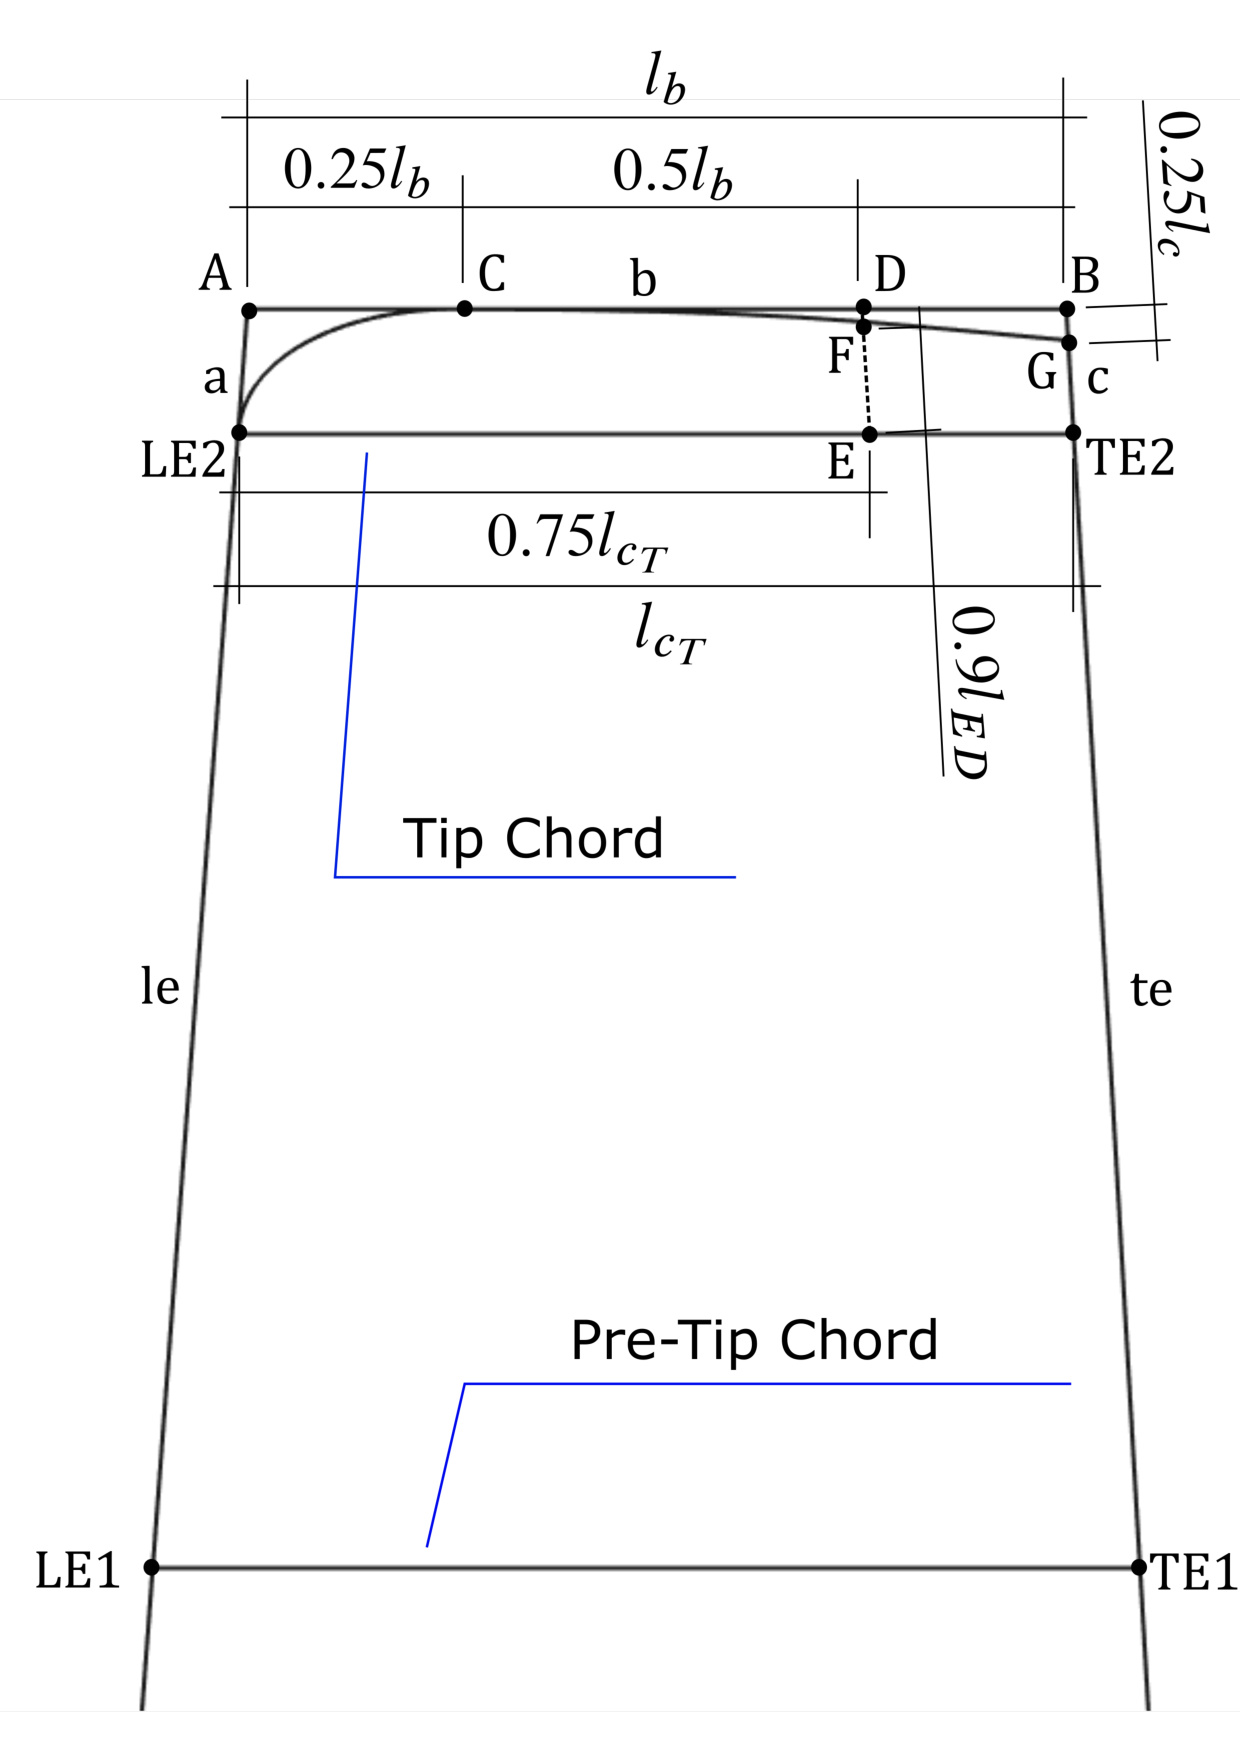
\includegraphics[scale=0.42]{Immagini/Capitolo3/wingtip_1}
\caption{Wing tip construction plane, complete with point definitions and edge dimensions}
\label{fig:WingTip1}
\end{figure}
% 
\begin{figure}[H]
\centering
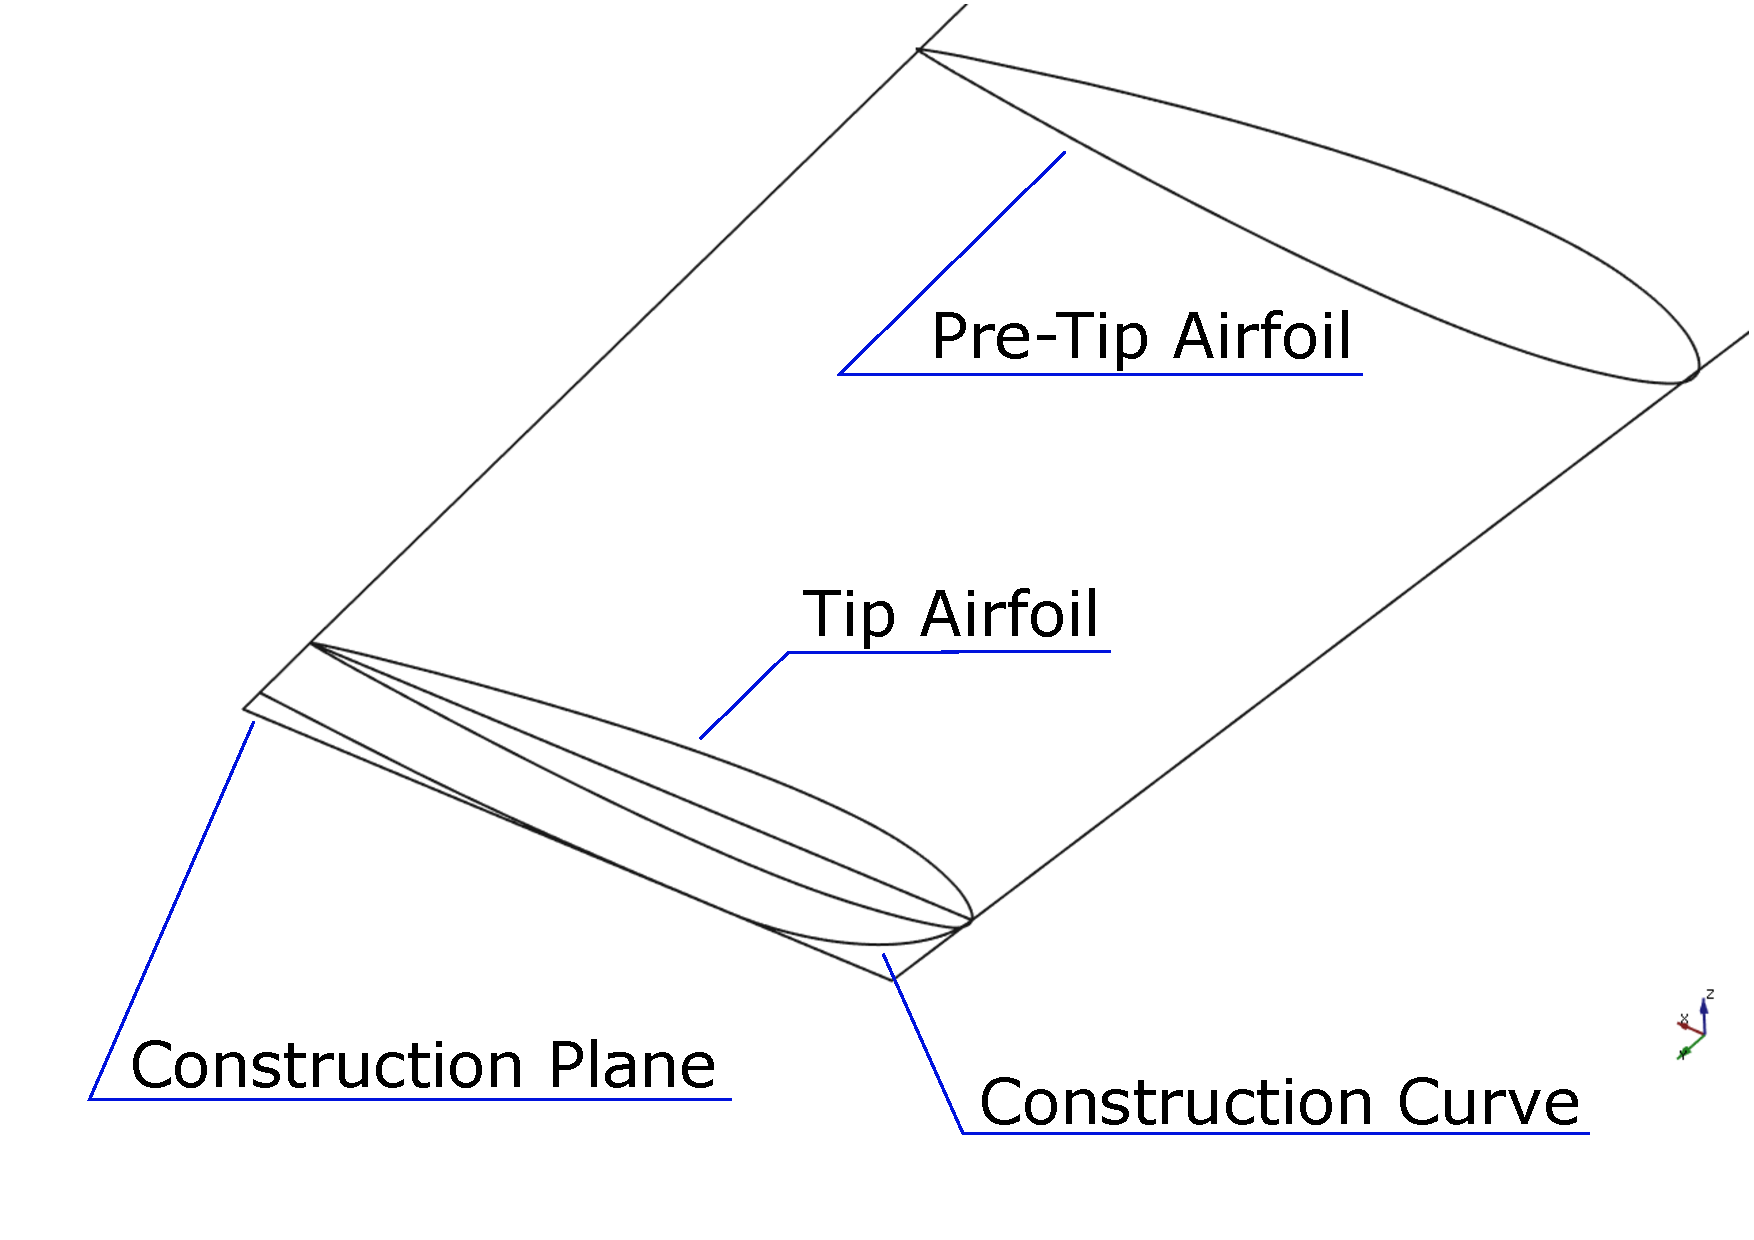
\includegraphics[scale=0.37]{Immagini/Capitolo3/wingtip_2}
\caption{Wing tip in-plane construction curve}
\label{fig:WingTip1}
\end{figure}
% 

\bigskip
\noindent
The in-plane construction curves serve as some sort of guide for the actual supporting curves of the wing tip, by providing points for their construction. First cross section curves to be generated are those passing for the points C, F, and G. \lstinline[language=Java]!AircraftUtils! contains a private static method, called \lstinline[language=Java]!createVerCrvsForTipClosure!, that generates cross section curves for the tip (in the form of \lstinline[language=Java]!CADGeomCurve3D! objects) by means of the following arguments:
%
\begin{itemize}
\item an instance of the \lstinline[language=Java]!LiftingSurface! class representing the lifting surface;
\item two Java \gls{List}s of \lstinline[language=Java]!OCCEdge! objects, containing respectively the upper and the lower edges of the tip and pre-tip airfoil;
\item two \lstinline[language=Java]!PVector! entities, representing the directions of the leading and trailing edge of the wing wireframe, respectively;
\item a \lstinline[language=Java]!double! entry, whose value is between $0.0$ and $1.0$, and states at which station, in terms of the tip chord fraction, the supporting curve needs to be created;
\item 3D point coordinates in the form of a \lstinline[language=Java]!double! array, representing the point on the in-plane construction curve that the supporting curve needs to pass through.
\end{itemize}
%
This algorithm uses the entries listed above in order to build curves that start on the upper side of the wing tip airfoil and end on the lower one, passing through the in-plane construction curve. In order to get the necessary points on the tip airfoil curves, the method makes use of the \lstinline[language=Java]!PVector! \lstinline[language=Java]!cross! static function, which allows to calculate the cross product between vectors. The cross product one is interested in in this case is the one between the vector representing the chord (or a fraction of it) of the wing tip airfoil and one of the vectors belonging to the construction plane (such as the leading and trailing edge vectors passed to the method), in order to generate segments belonging to the tip airfoil plane and perpendicular to its chord. These segments are then used to calculate points on the airfoil curves, once being multiplied by a scalar quantity representing the semi-airfoil (upper or lower side) height with respect to its chord. These scalar quantities are provided by a private static method, still contained in \lstinline[language=Java]!AircraftUtils! and called \lstinline[language=Java]!getThicknessAtX!, which requires an object belonging to the \gls{JPAD} \lstinline[language=Java]!Airfoil! class (representing the basic airfoil) and a \lstinline[language=Java]!double! value standing for the chord fraction at which the heights (both in the up and down direction) of the airfoil curve must be calculated. The segments, once scaled, finally provide the points on the airfoil curve, by means of the static method \lstinline[language=Java]!pointProjectionOnCurve! contained in \lstinline[language=Java]!OCCUtils!. 

\bigskip
\noindent
Points are not the only thing needed in order to generate the cross section curves of the wing tip. Three tangency constraints need to be imposed onto these curves: one at the starting point, on the upper side of the tip profile; the second one at the intersection with the in-plane curve; the last one at the ending point, on the lower side of the tip curve. These tangency constraints (the first and the last one in particular) are calculated still by means of the curves of the last and penultimate airfoils. In fact, in order to obtain a smooth transition from the last panel shell to the one of the wing tip, tangent vectors are calculated by simply connecting corresponding points (i.e., points located at the same chord fraction) onto the penultimate and last airfoil. Points on the pre-tip airfoil curve are calculated in the same way as described above. Regarding the second tangent vector, instead, it is simply imposed coincident with the normal vector of the wing tip construction plane. In order to obtain the right shape for the supporting curves, tangent vector magnitudes are adjusted according to some parameters, which depend on the tip airfoil thickness and on the distance between the in-plane construction curve and tip airfoil plane at the cross section at which the curve is being calculated. The piece of code below (listing \ref{lst:TipSupCurves}) just gives a glimpse at the operations behind the search of the appropiate magnitudes for the tangent vectors. Once all these operations are accomplished, the algorithm finally performs the curves calculation. For the same reasons specified above, the code produces two supporting curves at a time, that are collected into a \lstinline[language=Java]!CADGeomCurve3D! array and returned to the calling method. Figure \ref{fig:WingTip1} shows the result obtained at this stage.
%
\bigskip
\begin{lstlisting}[caption={Tip supporting curves tangent vectors magnitudes}, captionpos=b, tabsize=2, label={lst:TipSupCurves}]
// Determine tip airfoil thicknesses with respect to its chord segment
double thickUpp = PVector.sub(pntOnTipAirfoilUCrv, pntOnTipChord).mag();
double thickLow = PVector.sub(pntOnTipAirfoilLCrv, pntOnTipChord).mag();

// Determine construction curve height with respect to
// the tip airfoil chord segment
double crvHeight = PVector.sub(
		new PVector(
				(float) guideCrvPnt[0], 
				(float) guideCrvPnt[1], 
				(float) guideCrvPnt[2]), 		
		pntOnTipChord).mag(); 

// Determine tangent magnitudes, both for the upper and lower
// supporting curves, based on the just calculated values	
double tanUppVSecCrvFac = 1;
double tanLowVSecCrvFac = 1*(-1);		
double tanUppHalfVSecCrvFac = Math.pow(thickUpp/crvHeight, 0.60)*(-1); 
double tanLowHalfVSecCrvFac = Math.pow(thickLow/crvHeight, 0.60)*(-1);
\end{lstlisting}
% 
\begin{figure}[H]
\centering
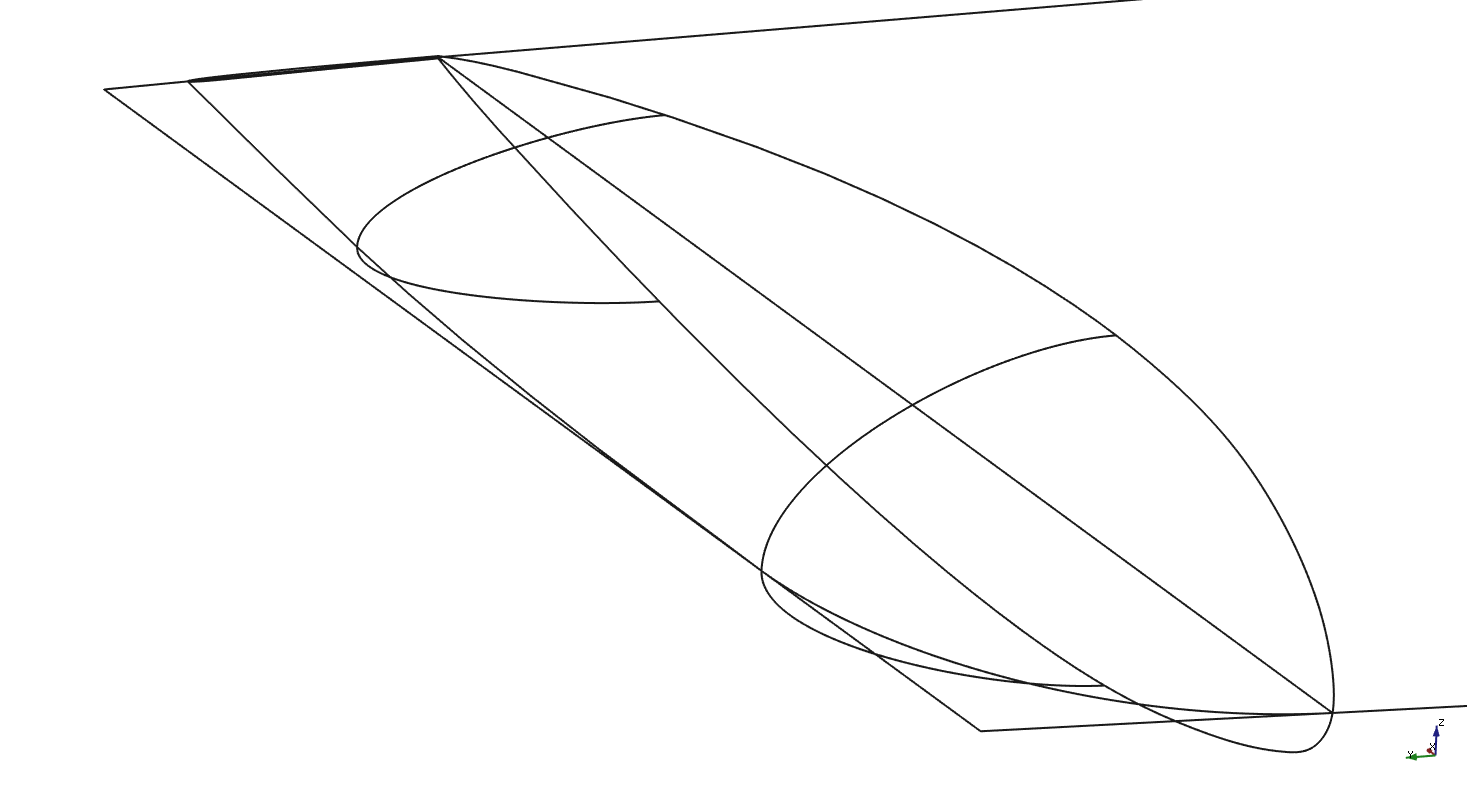
\includegraphics[scale=0.40]{Immagini/Capitolo3/WingTipWireframeMainSections}
\caption{Wing tip wireframe main supporting curves}
\label{fig:WingTip1}
\end{figure}
% 

\bigskip
\noindent
For the main supporting curves, namely those crossing the tip airfoil at the $25\%$, $75\%$ and $100\%$ in terms of its chord fraction, it is not necessary to calculate anything for the last entry of the \lstinline[language=Java]!createVerCrvsForTipClosure! method, since those points are the ones that have been used to determine the shape of the in-plane construction curve. When it comes to supporting curves between the main ones (which are necessary in order to make sure the tip patching process is successfully accomplished) some calculation is needed instead. First thing, spacings between these curves are established by means of three arrays (reported in listing \ref{lst:TipSubSupCurves}), one for each of the sections the wing tip has been split into by the previous step. These spacings are used directly to determine points on the in-plane construction curves by employing their parametric definition and their range. But once these points have been successfully obtained, what it is necessary to do, in order to use the same method described above in order to generate cross section curves, is determine their position in terms of wing tip chord fraction. This operation is quite simple to accomplish and involves just linear interpolation (provided by the \gls{JPAD} utility class \lstinline[language=Java]!MyMathUtils!) and some basic geometry consideration, and is reported in listing \ref{lst:TipSubSupCurves}. Once the necessary chord fractions have been obtained, the \lstinline[language=Java]!createVerCrvsForTipClosure! method can be used, and the resulting cross section curves are arranged in three different arrays, in order to be used later in the code. The \lstinline[language=Java]!double! arrays defining these sections follow a peculiar spacing, especially for the first one. These spacings have been chosen after performing several tests, while searching for the best results in terms of returned shapes. Figure \ref{fig:WingTip2} shows the final result for the wing tip wireframe.
%
\bigskip
\begin{lstlisting}[caption={Supporting curves between main wing tip cross sections}, captionpos=b, tabsize=2, label={lst:TipSubSupCurves}]
// Sub cross sections arrays		
double[] subVSecP1Vector = {0.10, 0.15, 0.40, 0.55, 0.60, 0.75, 0.90}; 
double[] subVSecP2Vector = {0.25, 0.50, 0.75};
double[] subVSecP3Vector = {0.25, 0.50, 0.75};

List<double[]> subVSecVector = new ArrayList<>();

subVSecVector.add(subVSecP1Vector);
subVSecVector.add(subVSecP2Vector);
subVSecVector.add(subVSecP3Vector);
				
List<CADGeomCurve3D[]> subVSecP1 = new ArrayList<>();
List<CADGeomCurve3D[]> subVSecP2 = new ArrayList<>();
List<CADGeomCurve3D[]> subVSecP3 = new ArrayList<>();	
List<List<CADGeomCurve3D[]>> subVSec = new ArrayList<List<CADGeomCurve3D[]>>();

// Iterate through the wing tip sections, in order 
// to generate additional  supporting curves
for(int i = 0; i < 3; i++) {
	int idx = i;
	subVSec.add(Arrays
		.stream(subVSecVector.get(i))
		.mapToObj(f -> {
			double[] crvRange = constrPlaneGuideCrvs.get(idx).getRange();
			double[] pntOnGuideCurve = constrPlaneGuideCrvs.get(idx)
							.value(f*(crvRange[1]-crvRange[0])+crvRange[0]);
			double interpCoord;
			double chordFraction;
			double x = pntOnGuideCurve[0];
			
			// Determine the corresponding chord fraction for the just  
			// calculated point lying on the construction curve
			if(!typeLS.equals(ComponentEnum.VERTICAL_TAIL)) {
				interpCoord = pntOnGuideCurve[1];
				double xLE = MyMathUtils.getInterpolatedValue1DLinear(
					new double[] {le2.y, aPnt.y}, 
					new double[] {le2.x, aPnt.x}, 
					interpCoord
			    		);
			    	double xTE = MyMathUtils.getInterpolatedValue1DLinear(
			    		new double[] {te2.y, bPnt.y}, 
			    		new double[] {te2.x, bPnt.x}, 
			    		interpCoord
			    		);
			    	chordFraction = (x - xLE)/(xTE - xLE);
			} else {
			    	interpCoord = pntOnGuideCurve[2];
			    	double xLE = MyMathUtils.getInterpolatedValue1DLinear(
			    		new double[] {le2.z, aPnt.z}, 
			    		new double[] {le2.x, aPnt.x}, 
			    		interpCoord
			    		);
			    	double xTE = MyMathUtils.getInterpolatedValue1DLinear(
			    		new double[] {te2.z, bPnt.z}, 
			    		new double[] {te2.x, bPnt.x}, 
			    		interpCoord
			    		);
			    	chordFraction = (x - xLE)/(xTE - xLE);
			}
			
			// Generate the supporting curve
			CADGeomCurve3D[] subVSecCrvs = createVerCrvsForTipClosure(
			    	liftingSurface, 
			    	airfoilTipCrvs,
			    	airfoilPreTipCrvs,
			    	new PVector[] {le1, le2},
			    	new PVector[] {te1, te2},
			    	chordFraction,
			    	pntOnGuideCurve
			    	);
			 return subVSecCrvs;
		})
		.collect(Collectors.toList())
		);
}

// Collect the additional supporting curves in three different arrays
subVSecP1.addAll(subVSec.get(0));
subVSecP2.addAll(subVSec.get(1));
subVSecP3.addAll(subVSec.get(2));
\end{lstlisting}
% 
\begin{figure}[H]
\centering
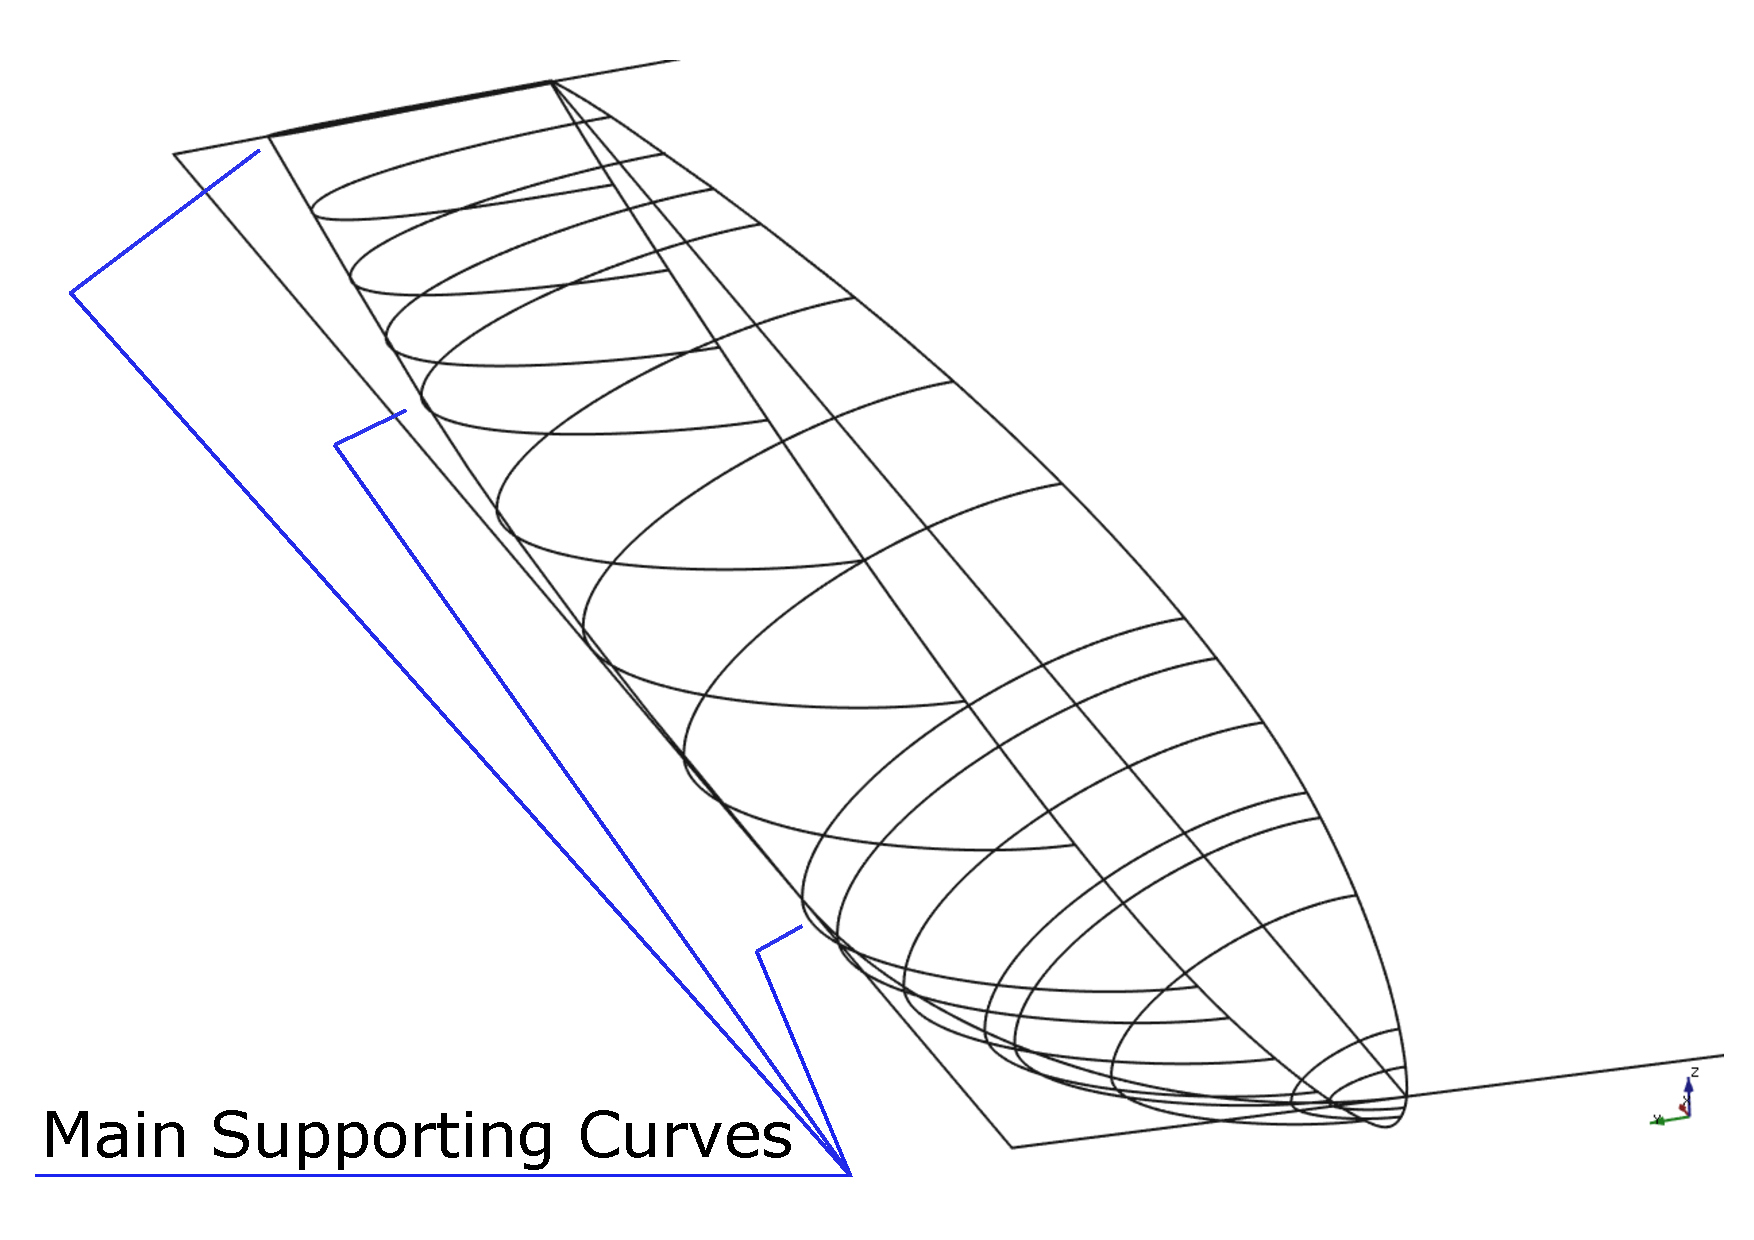
\includegraphics[scale=0.35]{Immagini/Capitolo3/wingtip_4}
\caption{Wing tip wireframe supporting curves}
\label{fig:WingTip2}
\end{figure}
% 

\bigskip
\noindent
Once the definitive wireframe has been built, it is finally possible to generate wing patches. The first ones to be created are those for the wing panels. The procedure is quite similar to the one used for the fuselage. The aforementioned list of lists, called \lstinline[language=Java]!cadCurveAirfoilList! and containing \lstinline[language=Java]!CADGeomCurve3D! entities representing airfoil curves, is used along with the \lstinline[language=Java]!makePatchThruSections! method in order to generate a loft for each panel. The piece of code below briefly explains the procedure, while figure \ref{fig:WingPanelPatches} depicts the results.
%
\bigskip
\begin{lstlisting}[caption={Spacings for supporting curves between main wing tip cross sections}, captionpos=b, tabsize=2, label={lst:TipSubSupCurves}]
List<OCCShape> patchWing = new ArrayList<>();
patchWing.addAll(cadCurveAirfoilList.stream()
		                   .map(OCCUtils::makePatchThruSections)
		                   .collect(Collectors.toList()));
\end{lstlisting}
% 
\begin{figure}[H]
\centering
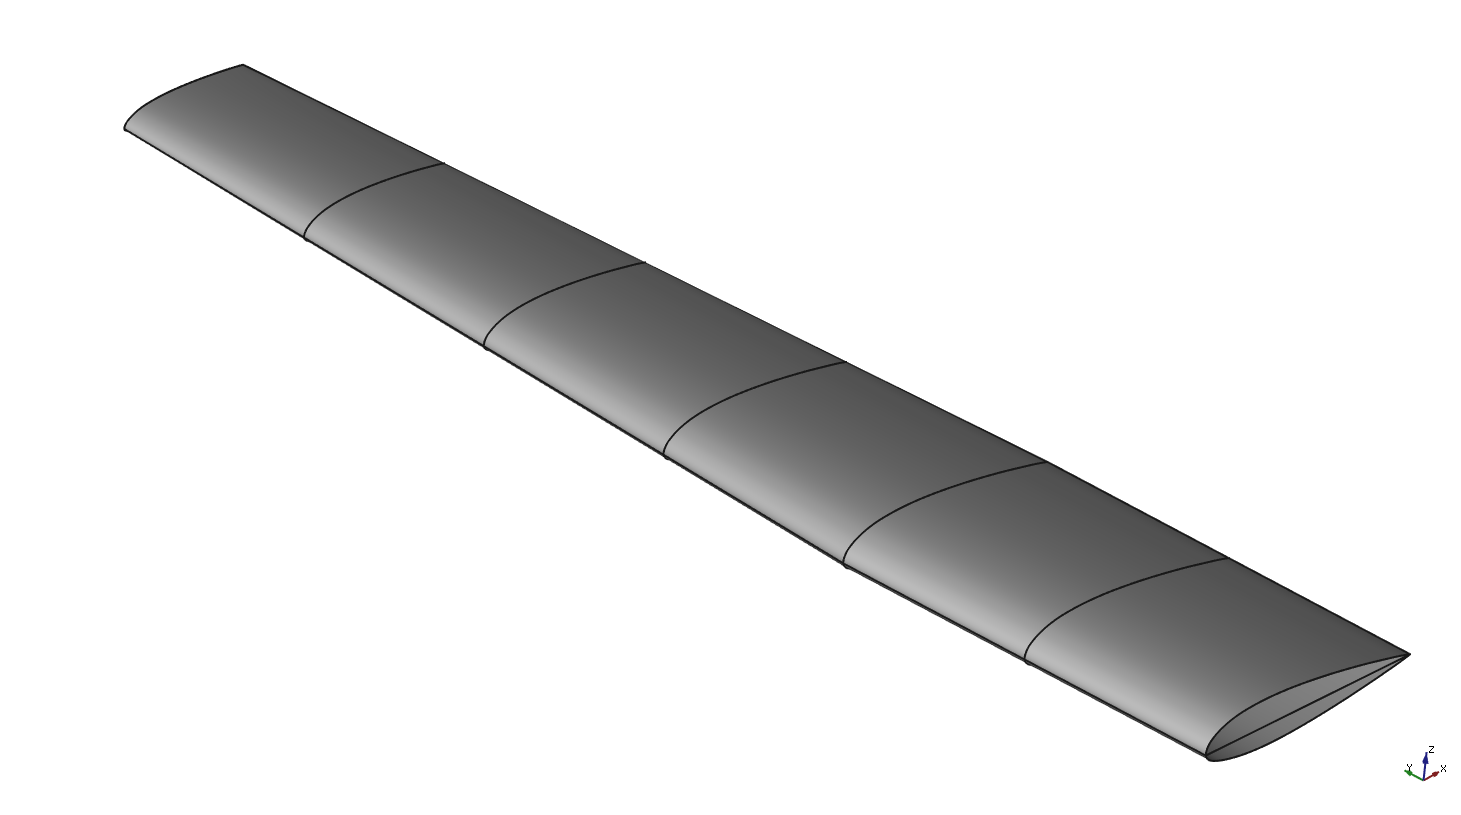
\includegraphics[scale=0.40]{Immagini/Capitolo3/WingPatches}
\caption{Main wing patches}
\label{fig:WingPanelPatches}
\end{figure}
% 

\bigskip
\noindent
Then it's the turn for the wing tip. The patching process can be divided in four stages, with the first one regarding the forward part of the wing tip. In order to obtain a smoother surface than the one that would be returned by simply using the \lstinline[language=Java]!makePatchThruSections! algorithm (the one involving curves and vertices), it has been decided to employ a different method and some different \gls{OCCT} classes. In particular, the choice has fallen on the \lstinline[language=Java]!BRepOffsetAPI_MakeFilling! class, which allows to generate filling surfaces by providing a set of curves bounding the face we want to generate, and a set of points defining some constraints the support face has to satisfy. In order to provide the bounding edges the algorithm requires, it has been necessary to split the first of the in-plane construction curves and the upper and lower curves defining the wing tip airfoil at the extremities of the second pair of supporting curves of the wing tip wireframe first section. This task has been accomplished by means of the \lstinline[language=Java]!OCCUtils! \lstinline[language=Java]!splitEdge! method. Then several points on the first of the supporting curves have been used as constraints for the final surface. In order to obtain the best result possible, two filling surfaces have actually been created, one for the upper side and one for the lower one. The following listing shows how the procedure has been coded, while figure \ref{fig:WingTipFilling} shows the final result.
%
\bigskip
\begin{lstlisting}[caption={Wing tip leading edge filling code, upper side}, captionpos=b, tabsize=2, label={lst:WingTipFilling}]
// Splitting the tip airfoil curves and the construction  
// curve #1 in order to fill the wing tip LE correctly
List<OCCEdge> airfoilUpperCrvs = new ArrayList<>();
airfoilUpperCrvs.addAll(OCCUtils.splitEdge(
		OCCUtils.theFactory.newCurve3D(airfoilTipCrvs.get(0)), 
		subVSecP1.get(1)[0].edge().vertices()[0].pnt()
		));
		
List<OCCEdge> constPlaneGuideCrvs1 = new ArrayList<>();
constPlaneGuideCrvs1.addAll(OCCUtils.splitEdge(
		constrPlaneGuideCrv1, 
		subVSecP1.get(1)[0].edge().vertices()[1].pnt()
		));

// Creating a filler surface at the wing tip leading edge, upper side.
// The procedure for the lower side pretty identical.			
double[] contrCrvUppRng = subVSecP1.get(0)[0].getRange();
double[] contrPntUpp1 = subVSecP1.get(0)[0].value(
		0.25*(contrCrvUppRng[1] - contrCrvUppRng[0]) + contrCrvUppRng[0]);
double[] contrPntUpp2 = subVSecP1.get(0)[0].value(
		0.50*(contrCrvUppRng[1] - contrCrvUppRng[0]) + contrCrvUppRng[0]);
double[] contrPntUpp3 = subVSecP1.get(0)[0].value(
		0.75*(contrCrvUppRng[1] - contrCrvUppRng[0]) + contrCrvUppRng[0]);

BRepOffsetAPI_MakeFilling fillerP1Upp = new BRepOffsetAPI_MakeFilling();

fillerP1Upp.Add(
		airfoilUpperCrvs.get(1).getShape(),
		GeomAbs_Shape.GeomAbs_C0);
fillerP1Upp.Add(
		((OCCEdge)((OCCGeomCurve3D)subVSecP1.get(1)[0]).edge()).getShape(),
		GeomAbs_Shape.GeomAbs_C0);
fillerP1Upp.Add(
		constPlaneGuideCrvs1.get(0).getShape(),
		GeomAbs_Shape.GeomAbs_C0);		

fillerP1Upp.Add(new gp_Pnt(contrPntUpp1[0], contrPntUpp1[1], contrPntUpp1[2]));
fillerP1Upp.Add(new gp_Pnt(contrPntUpp2[0], contrPntUpp2[1], contrPntUpp2[2]));
fillerP1Upp.Add(new gp_Pnt(contrPntUpp3[0], contrPntUpp3[1], contrPntUpp3[2]));

fillerP1Upp.Build();
\end{lstlisting}
% 
\bigskip
\begin{figure}[H]
\centering
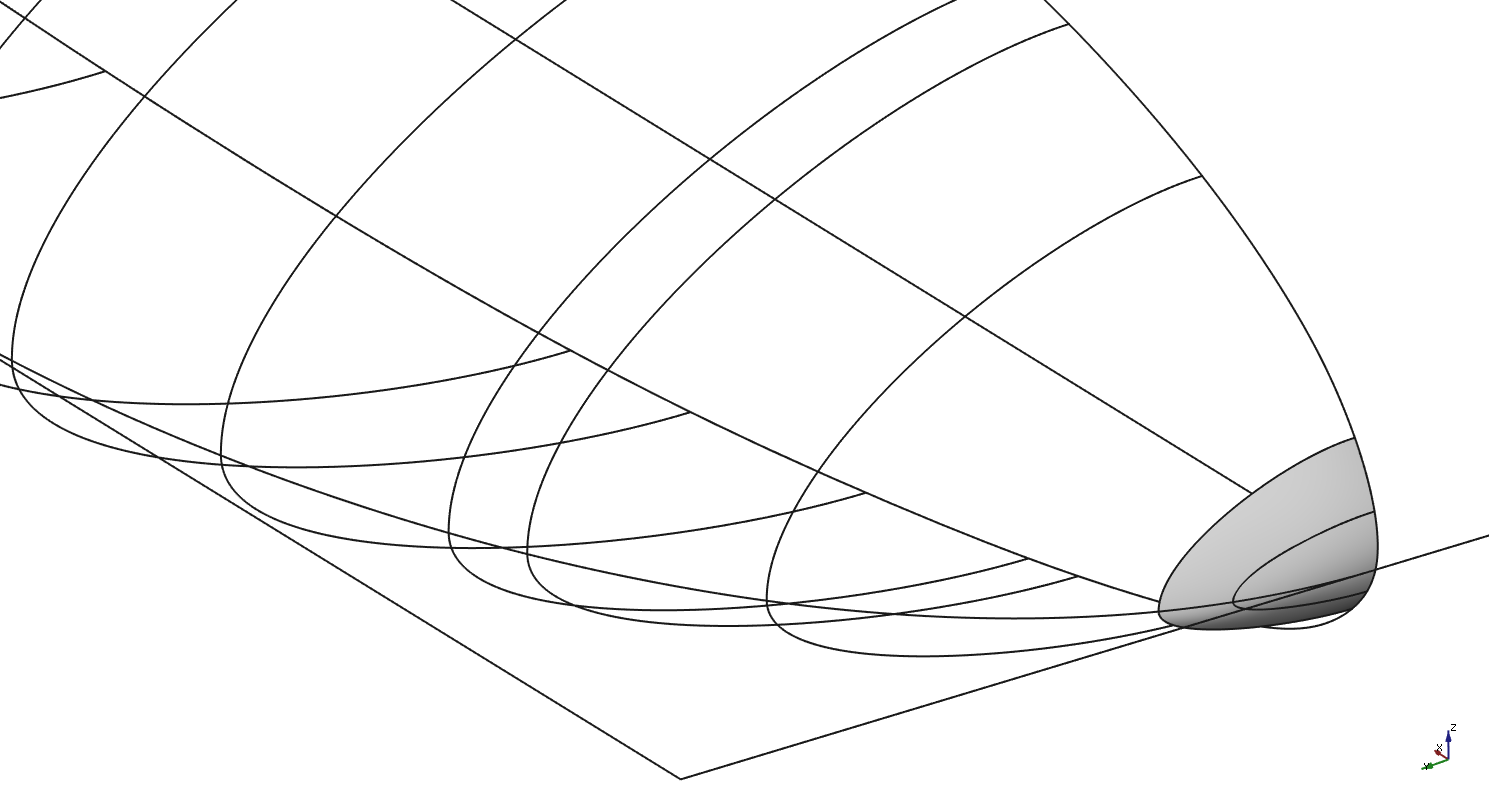
\includegraphics[scale=0.35]{Immagini/Capitolo3/WingTipLEFilling}
\caption{Wing tip leading edge filling surface}
\label{fig:WingTipFilling}
\end{figure}
%  

\bigskip
\noindent
The remaining sections of the wing tip are completed by means of the \lstinline[language=Java]!makePatchThruSections! algorithm. It has to be said that the second section (the one going from point C to point F, to be clear), has not been obtained in a single step (i.e., by patching through all the cross sections at the same time), but splitting the patching in two, in order to obtain the best result. This is the reason why, in the figures in which the final shell and solid shapes are depicted, the wing tip shell presents five patches rather than four, including the one obtained by the use of the filling algorithm. Figure \ref{fig:WingTipFinal} shows all the patches along with the supporting curves.
% 
\begin{figure}[H]
\centering
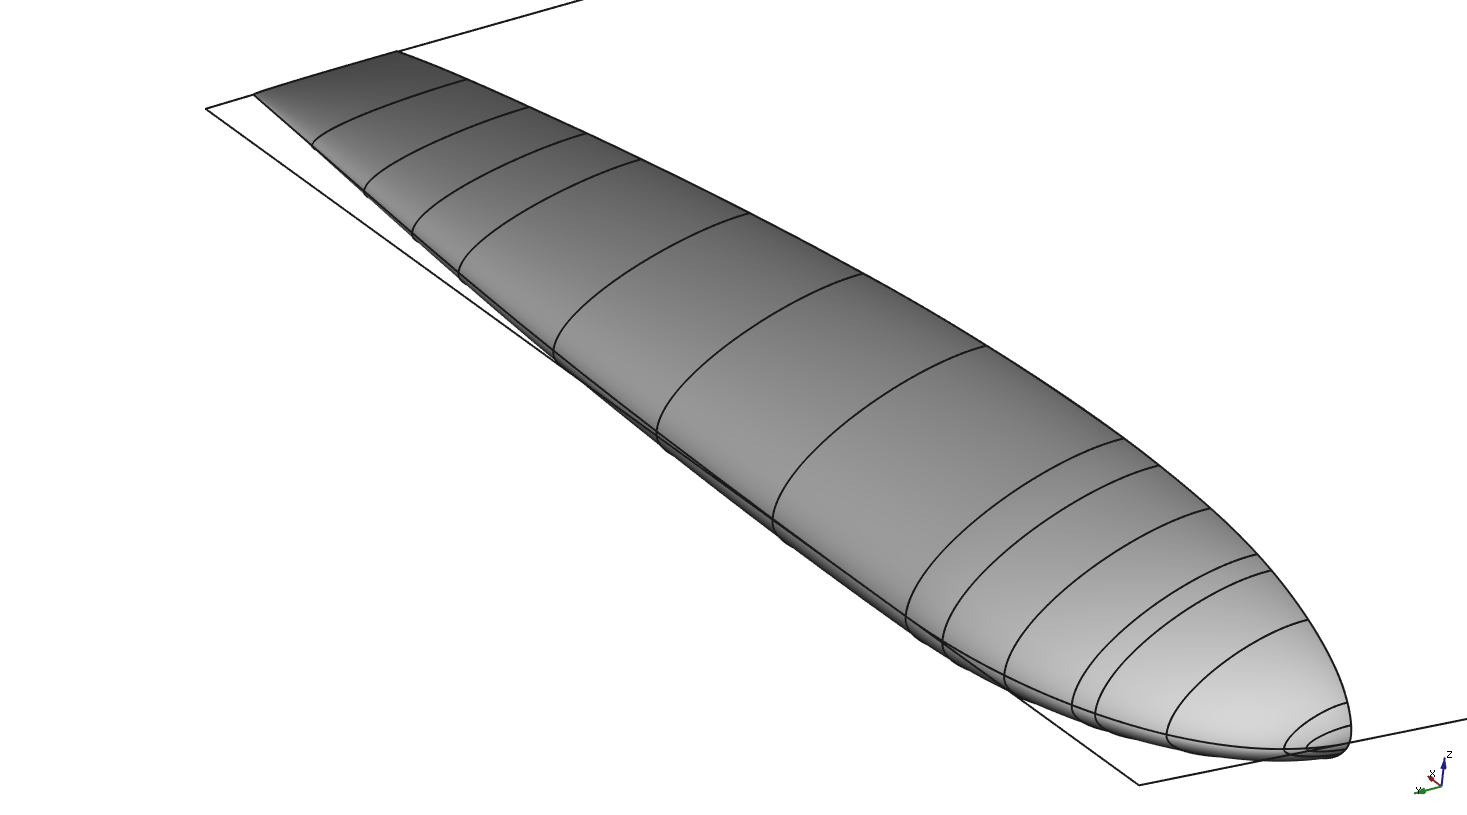
\includegraphics[scale=0.38]{Immagini/Capitolo3/WingTipPatches}
\caption{Wing tip patches and supporting curves}
\label{fig:WingTipFinal}
\end{figure}
%  

\bigskip
\noindent
Before sewing all the patches together in order to obtain one single shell, another step is needed. In fact, the aforementioned operation performed by the \lstinline[language=Java]!populateCoordinateList! method, consisting in opening the trailing edge of the airfoil whether necessary, has left some sort of hole on the back of the wing that must be filled. This operation has to be performed both for the panel patches and the wing tip, and the method that allows to do this is one of those listed in Chapter \ref{chap2}: the \lstinline[language=Java]!OCCUtils! static method \lstinline[language=Java]!makeFilledFace!. The \gls{OCCT} algorithm behind this method is provided by the same class used above, in order to fill the leading edge of the wing tip: \lstinline[language=Java]!BRepOffsetAPI_MakeFilling!. However, the way the algorithm is implemented in \lstinline[language=Java]!OCCUtils! allows just to determine the flat surface bounded by the curves the method is provided with. So, the method accepts an array of indefinite length of \lstinline[language=Java]!CADGeomCurve3D! entities, and returns the surface between the curves (which necessaryly must provide a closed wire). Figure \ref{fig:WingTipTE} shows the filling surface for the trailing edge of the wing tip.
% 
\begin{figure}[H]
\centering
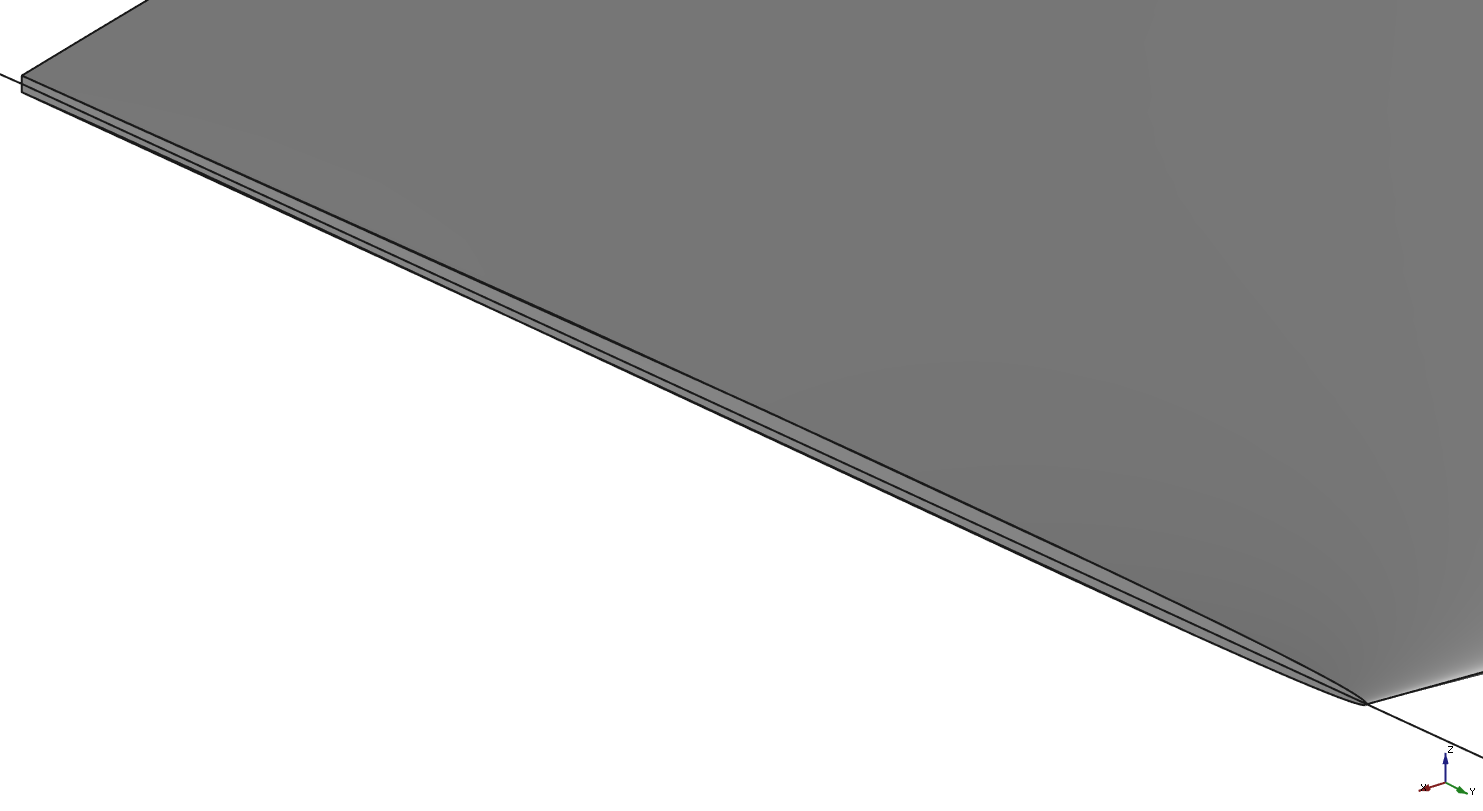
\includegraphics[scale=0.30]{Immagini/Capitolo3/WingTipTEFilledFace}
\caption{Wing tip trailing edge filling surface}
\label{fig:WingTipTE}
\end{figure}
%  

\bigskip
\noindent
The next steps consist in sewing all the patches and the faces created till now. First, wing panel patches are sewed, along with the trailing edge filling surfaces mentioned above. Then it is necessary to sew together the wing tip patches. This operation is much more delicate than the preceding one, since in this case the curves that define the borders of the patches we want to sew do not exactly coincide. This is due to the use of the edge splitting algorithm, which sligthly modify the returning curves respect to the original one. In order to overcome this problem, the default tolerance of the sewing algorithm has been changed, and set to the value which is provided as input to the \lstinline[language=Java]!getLiftingSurfaceCAD! method. For the same reasons, the default tolerance for the sewing algorithm needs to be set to a different (higher) value when sewing the wing tip shell with the one obtained by sewing the panel lofts. In this case, in particular, the difference between the two shells is much more evident, due to the fact that they have been obtained by patching through sections following different (orthogonal) directions.

\bigskip
\noindent
The following operations are pretty much the same conducted for the fuselage solid construction. The main difference consists in the fact that mirroring operations are not necessary in case the lifting surface is a vertical tail. In fact, in this case, the only necessary operation consists in closing the side of the shell which is still open (i.e., the side opposite to the one where the wing tip has been built). The following piece of code (listing \ref{lst:VerticalTailClosing}) shows how this operation has been implemented in the \lstinline[language=Java]!getLiftingSurfaceCAD! algorithm. Again, the method this operation makes use of is the \lstinline[language=Java]!OCCUtils! static function \lstinline[language=Java]!makeFilledFace!.
%
\bigskip
\begin{lstlisting}[caption={Vertical tail filling operations}, captionpos=b, tabsize=2, label={lst:VerticalTailClosing}]
// Check whether the lifting surface is a vertical tail
if(typeLS.equals(ComponentEnum.VERTICAL_TAIL)) {
		CADShape faceRoot = OCCUtils.makeFilledFace(
		
		 		// Get the first of the airfoil curves
				cadCurveAirfoilList.get(0).get(0),  
				
				// Create a segment representing the trailing
				// edge of the first of the airfoil curves
				OCCUtils.theFactory.newCurve3D( 
						cadCurveAirfoilList.get(0).get(0).edge().vertices()[0].pnt(), 
						cadCurveAirfoilList.get(0).get(0).edge().vertices()[1].pnt()
						) 
				);
				
		// Add this shape to the ones to be sewed	
		sewMakerWing.Add(((OCCShape) faceRoot).getShape()); 
}		
\end{lstlisting}

\bigskip
\noindent
In case the lifting surface is not a vertical tail, mirroring, sewing, and solid generating operations are performed by means of the same methods and classes listed above, for the fuselage \gls{CAD} problem. In this case too, the method allows to export just the desired shapes: by setting the previously mentioned \lstinline[language=Java]!boolean! arguments, the user can decide which types of shapes he wants to extract. Figure \ref{fig:WingSolid} shows the final result in terms of solid shapes. In particular, the depicted wing is the one of the ATR-72. The following paragraphs will also provide more examples of lifting surfaces produced by means of the same algorithm.
% 
\begin{figure}[H]
\centering
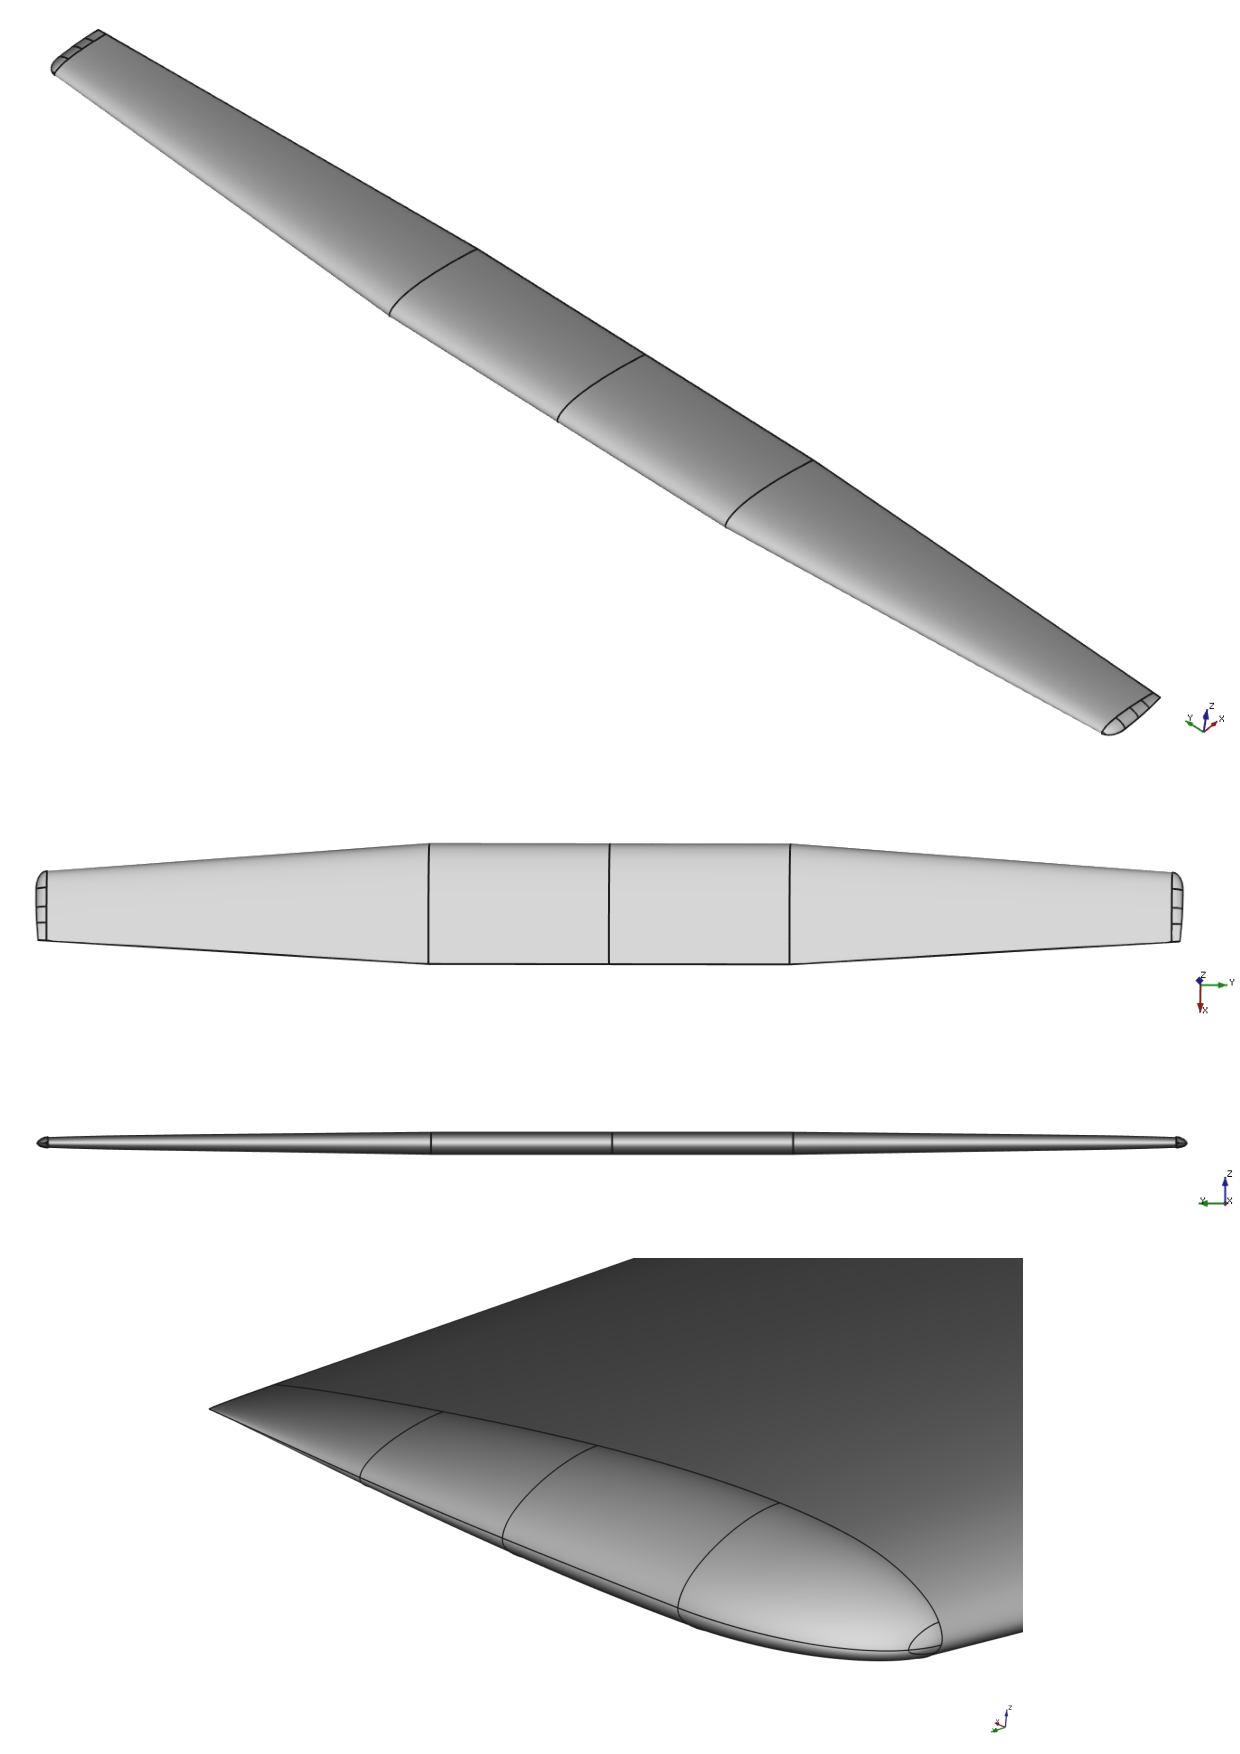
\includegraphics[scale=0.68]{Immagini/Capitolo3/wing_2}
\caption{ATR-72 solid wing, with a close-up on the wing tip}
\label{fig:WingSolid}
\end{figure}
%  

\section{\texttt{AircraftUtils} additional methods}
\label{sec3.5}
The methods analyzed in the previous paragraphs provide just the necessary tools to build \gls{CAD} shapes out of data stored in \gls{JPAD} aircraft classes. In order to actually be able to import aircraft data from files and write generated \gls{CAD} shapes to specific file formats, \lstinline[language=Java]!AircraftUtils! needs to be filled with additional methods. This paragraph gives an overview on the extra functions (and sub-classes) contained in \lstinline[language=Java]!AircraftUtils!, providing basic information on how they work and the classes they make use of.

\subsection{\texttt{importAircraft}}
\label{sec3.5.1}

The \lstinline[language=Java]!importAircraft! method is the tool that has been used in \lstinline[language=Java]!JPADCADSandbox! tests in order to actually import aircraft data from XML files and populate instances of the \gls{JPAD} \lstinline[language=Java]!aircraft! class. The operations performed by this method rely on an important Java library: \lstinline[language=Java]!args4j! \cite{args4j}. In short, \lstinline[language=Java]!args4j! library provides classes that allow to parse command line options. In this way, the paths to the directories and the files containing the necessary information to build new \lstinline[language=Java]!aircraft! instances can be easily managed and passed to the \gls{JPAD} utilities that provide support to XML file reading operations. In particular, the \lstinline[language=Java]!importAircraft! method accepts just one parameter, of the Java \lstinline[language=Java]!String[]! type, that contains the list of all the necessary directories. This list must be written according to the same notation used for the definition of the options of a supporting class (which in the present case has been called \lstinline[language=Java]!ArgumentsJPADCADSandbox!) that, along with the \lstinline[language=Java]!args4j! \lstinline[language=Java]!CmdLineParser! class, actually performs the parsing of the command line. Once the input array has been parsed, it is finally possible to populate the \lstinline[language=Java]!aircraft! object, by means of the \lstinline[language=Java]!JPADXmlReader! class. An example of usage of this method is given in paragraph \ref{sec3.6}.

\subsection{\texttt{enum} classes}
\label{sec3.5.2}

The \lstinline[language=Java]!AircraftUtils! class contains two Java \lstinline[language=Java]!enum! classes, which have yet been mentioned in the previous paragraphs. What follows focuses on their definitions and their usage.

\subsubsection{\texttt{FileExtension}}

This \lstinline[language=Java]!enum! class is used to enumerate all the possible file formats, supported by the \gls{OCCT} library, that can be used to save \gls{CAD} entities. In particular, this class is used by another \lstinline[language=Java]!AircraftUtils! method, which is explained just below, in order to select the right operations to perform for the purpose of writing \gls{CAD} shapes to a specific file format. Listing \ref{lst:FileExtension} reports the structure of this \lstinline[language=Java]!enum! class.
%
\bigskip
\begin{lstlisting}[caption={\lstinline!FileExtension! class}, captionpos=b, tabsize=2, label={lst:FileExtension}]
public enum FileExtension {
		BREP,
		STEP,
		IGES,
		STL;
}
\end{lstlisting}

\subsubsection{\texttt{XSpacingType}}

The \lstinline[language=Java]!XSpacingType! class is used to enumerate the spacings that it is possible to employ once being provided an interval and the number of points that must be contained in the interval. In addition to the definitions of the elements of the class, it also contains an abstract method, named \lstinline[language=Java]!calculateSpacing!, that it is implemented by each one of the enumerators (listing \ref{lst:XSpacingType}). This \lstinline[language=Java]!enum! class is used by the \lstinline[language=Java]!getFuselageCAD! method in order to define the spacing for the cross sections of the nose and the tail trunks.
%
\bigskip
\begin{lstlisting}[caption={\lstinline!XSpacingType! class}, captionpos=b, tabsize=2, label={lst:XSpacingType}]
public enum XSpacingType {
		UNIFORM {
				@Override
				public Double[] calculateSpacing(double x1, double x2, int n) {
						Double[] xSpacing = MyArrayUtils.linspaceDouble(x1, x2, n);
						return xSpacing;
				}
		},
		COSINUS {
				@Override
				public Double[] calculateSpacing(double x1, double x2, int n) {
						Double[] xSpacing = MyArrayUtils.cosineSpaceDouble(x1, x2, n);
						return xSpacing;
				}
		},
		HALFCOSINUS1 { // finer spacing close to x1
				@Override
				public Double[] calculateSpacing(double x1, double x2, int n) {
						Double[] xSpacing = MyArrayUtils.halfCosine1SpaceDouble(x1, x2, n);
						return xSpacing;
				}
		}, 
		HALFCOSINUS2 { // finer spacing close to x2
				@Override
				public Double[] calculateSpacing(double x1, double x2, int n) {
						Double[] xSpacing = MyArrayUtils.halfCosine2SpaceDouble(x1, x2, n);
						return xSpacing;
				}
		}; 
		
		public abstract Double[] calculateSpacing(double x1, double x2, int n);
}
\end{lstlisting}

\subsection{CAD methods overload}
\label{sec3.5.3}

One of the most important characteristics of a language such as Java is the possibility to perform methods overloading. Method overloading is a feature that allows a class to have more than one method having the same name, if their argument lists are different. For this reason, it is possible to define various \lstinline[language=Java]!getLiftingSurfaceCAD! and \lstinline[language=Java]!getFuselageCAD!, differing from each other for the arguments they support. The following listing reports all the different versions for the aforementioned methods currently contained in \lstinline[language=Java]!AircraftUtils!.
\bigskip
\begin{lstlisting}[caption={CAD generating methods overloading in \lstinline!AircraftUtils!}, captionpos=b, tabsize=2, label={lst:MethodOverloading}]
public static List<OCCShape> getFuselageCAD(Fuselage fuselage,
			double noseCapSectionFactor1, double noseCapSectionFactor2, 
			int numberNoseCapSections, 
			int numberNosePatch2Sections, XSpacingType spacingTypePatch2, 
			int numberTailPatchSections, XSpacingType spacingTypeTailPatch, 
			double tailCapSectionFactor1, double tailCapSectionFactor2, 
			int numberTailCapSections,
			boolean exportLofts, boolean exportSolids, boolean exportSupportShapes) {
			
			...
}

public static List<OCCShape> getFuselageCAD(Fuselage fuselage, 
			boolean exportSupportShapes) {

		return getFuselageCAD(fuselage, 
				0.15, 1.0, 3, 
				7, XSpacingType.COSINUS, 
				7, XSpacingType.COSINUS, 
				1.0, 0.15, 3, 
				true, true, exportSupportShapes);
}

public static List<OCCShape> getFuselageCAD(Fuselage fuselage, 
			boolean exportLofts, boolean exportSolids, boolean exportSupportShapes) {
			
		return getFuselageCAD(fuselage, 
				0.15, 1.0, 3, 
				7, XSpacingType.COSINUS, 
				7, XSpacingType.COSINUS, 
				1.0, 0.15, 3, 
				exportLofts, exportSolids, exportSupportShapes);
}

public static List<OCCShape> getFuselageCAD(Fuselage fuselage, 
			int numberNosePatch2Sections, int numberTailPatchSections, 
			boolean exportLofts, boolean exportSolids, boolean exportSupportShapes) {
		
		return getFuselageCAD(fuselage,
				0.15, 1.0, 3,
				numberNosePatch2Sections, XSpacingType.COSINUS,
				numberTailPatchSections, XSpacingType.COSINUS,
				1.0, 0.15, 3, 
				exportLofts, exportSolids, exportSupportShapes);
}

public static List<OCCShape> getLiftingSurfaceCAD(LiftingSurface liftingSurface, 
			ComponentEnum typeLS,
			double tipTolerance,
			boolean exportLofts,
			boolean exportSolids,
			boolean exportSupportShapes) {
			
			...
}

public static List<OCCShape> getLiftingSurfaceCAD(LiftingSurface liftingSurface, 
			ComponentEnum typeLS,
			boolean exportSupportShapes) {
		
		return getLiftingSurfaceCAD(liftingSurface,
				typeLS,
				1e-3,
				true,
				true,
				exportSupportShapes);
}
\end{lstlisting}

\bigskip
\noindent
\lstinline[language=Java]!AircraftUtils! also contains a method, called \lstinline[language=Java]!getAircraftShapes!, that allows to perform more than just one 
\gls{CAD} generating operation at a time, meaning that fuselage and lifting surface shapes can be generated at the same time by using one single method. In particular, the method accepts an object representing the aircraft, and a list containing values of the \gls{JPAD} \lstinline[language=Java]!ComponentEnum! class, specifying which type of shapes (i.e., fuselage, wing, tail, canard) must be produced. Then the method returns a list containing all the generated \lstinline[language=Java]!OCCShape! objects (listing \ref{lst:getAircraftShapes}).
\bigskip
\begin{lstlisting}[caption={\lstinline!getAircraftShapes! method}, captionpos=b, tabsize=2, label={lst:getAircraftShapes}]
public static List<OCCShape> getAircraftShapes(
			Aircraft theAircraft,
			List<ComponentEnum> components
			) {		
		List<OCCShape> allShapes = new ArrayList<>();
		
		if(theAircraft.getFuselage() != null && 
		   components.contains(ComponentEnum.FUSELAGE)) {
			allShapes.addAll(getFuselageCAD(theAircraft.getFuselage(), true));
		}		
		if(theAircraft.getWing() != null && 
		   components.contains(ComponentEnum.WING)) {
			allShapes.addAll(getLiftingSurfaceCAD(theAircraft.getWing(), 
				ComponentEnum.WING, 1e-3, true, true, true));
		}		
		if(theAircraft.getHTail() != null && 
		   components.contains(ComponentEnum.HORIZONTAL_TAIL)) {		
			allShapes.addAll(getLiftingSurfaceCAD(theAircraft.getHTail(), 
				ComponentEnum.HORIZONTAL_TAIL, 1e-3, true, true, true));
		}		
		if(theAircraft.getVTail() != null && 
		   components.contains(ComponentEnum.VERTICAL_TAIL)) {		
			allShapes.addAll(getLiftingSurfaceCAD(theAircraft.getVTail(), 
				ComponentEnum.VERTICAL_TAIL, 1e-3, true, true, true));
		}			
		if(theAircraft.getCanard() != null && 
		   components.contains(ComponentEnum.CANARD)) {		
			allShapes.addAll(getLiftingSurfaceCAD(theAircraft.getCanard(), 
				ComponentEnum.CANARD, 1e-3, true, true, true));
		}			
		return allShapes;
	}
\end{lstlisting}

\subsection{\texttt{getAircraftSolidFile}}
\label{sec3.5.4}

The \lstinline[language=Java]!getAircraftSolidFile! method allows to write solid shapes to file. It requires a Java \gls{List} containing generic \lstinline[language=Java]!OCCShape! entities, a \lstinline[language=Java]!String! standing for the name of the file we want to write, and an element of the \lstinline[language=Java]!FileExtension! class, which specifies the format of the file to be written. The first operation the method performs consists in filtering the input shapes, collecting all the solids found in one single list. This operation is made through the use of another \lstinline[language=Java]!AircraftUtils! static method, called \lstinline[language=Java]!getAircraftSolid!. Once all the solids have been obtained, the algorithm automatically chooses, by use of a switch statement, the right operations to perform in order to obtain a file in the format specified by the user. Currently the method supports writing in the following extensions:
%
\begin{itemize}
\item \gls{BRep},
\item STEP,
\item IGES,
\item STL.
\end{itemize}
%
All the writing operations rely on particular \gls{OCCT} classes, each one dedicated to a specific file format.

\section{Example}
\label{sec3.6}

The following example gives an idea of how the previously described methods can be used to automatically generate the \gls{CAD} model of an aircraft. For this purpose, a simple testing class has been created in \lstinline[language=Java]!JPADCADSandbox!. This class contains a main method that receives as input a \lstinline[language=Java]!String[]!, containing the paths to the directories that contain the XML files from which we want to read the aircraft data. The first operation consists in importing this data and fill in the \emph{fields} of a new \lstinline[language=Java]!Aircraft! object. This operation is conducted by using the \lstinline[language=Java]!importAircraft! method, by providing it with the aforementioned \lstinline[language=Java]!String! array. The next step consists in generating new instances of the \lstinline[language=Java]!Fuselage! and \lstinline[language=Java]!LiftingSurface! classes by making use of the methods of the \lstinline[language=Java]!Aircraft! class. Once they have been obtained, \gls{CAD} generating methods can be launched, by selecting one of the methods seen in section \ref{sec3.5.3}. In order to obtain the solid of the aircraft and write it to file (for the purpose of using it later, for example, in a \gls{CAD} or a \gls{CFD} software), the \lstinline[language=Java]!getAircraftSolidFile! method described above can be used, by providing it with the shapes we want to write, and the name and the format of the file (listing \ref{lst:Example01}).
%
\bigskip
\begin{lstlisting}[caption={Usage of \lstinline!AircraftUtils! methods}, captionpos=b, tabsize=2, label={lst:Example01}]
public class Test {

	public static void main(String[] args) {

		System.out.println("JPADCADSandbox Test");
		
		// Import aircraft data from XML files
		Aircraft aircraft = AircraftUtils.importAircraft(args);	
		
		// Generate instances of the JPAD 
		// classes describing aircraft components
		Fuselage fuselage = aircraft.getFuselage();	
		LiftingSurface wing = aircraft.getWing();		
		LiftingSurface hTail = aircraft.getHTail();
		LiftingSurface vTail = aircraft.getVTail();
		
		// Generate CAD shapes for all the aircraft components
		// and add them to a single List, in order to be exported
		List<OCCShape> allShapes = new ArrayList<>();
		
		List<OCCShape> fuselageShapes = AircraftUtils.getFuselageCAD(
				fuselage, 7, 7, true, true, true);
				
		List<OCCShape> wingShapes = AircraftUtils.getLiftingSurfaceCAD(
				wing, ComponentEnum.WING, 1e-3, true, true, true);
				
		List<OCCShape> hTailShapes = AircraftUtils.getLiftingSurfaceCAD(
				hTail, ComponentEnum.HORIZONTAL_TAIL, 1e-3, true, true, true);
				
		List<OCCShape> vTailShapes = AircraftUtils.getLiftingSurfaceCAD(
				vTail, ComponentEnum.VERTICAL_TAIL, 1e-3, true, true, true);	
				
		allShapes.addAll(fuselageShapes);
		allShapes.addAll(wingShapes);
		allShapes.addAll(hTailShapes);
		allShapes.addAll(vTailShapes);
		
		// Filter the shape list in order to collect the solid
		// ones only, and write them to STEP file format
		AircraftUtils.getAircraftSolidFile(allShapes, "aircraft", FileExtension.STEP);
	}
}
\end{lstlisting}

\bigskip
\noindent
Instead of generating \gls{CAD} shapes for each component at a time, one could have chosen to use the \lstinline[language=Java]!getAircraftShapes! method and provide it with the list of desired aircraft components (listing \ref{lst:Example02}). The results would have been exactly the same.
%
\bigskip
\begin{lstlisting}[caption={Usage of \lstinline!getAircraftShapes! method}, captionpos=b, tabsize=2, label={lst:Example02}]
		List<ComponentEnum> componentList = new ArrayList<>();
		componentList.add(ComponentEnum.FUSELAGE);
		componentList.add(ComponentEnum.WING);
		componentList.add(ComponentEnum.HORIZONTAL_TAIL);
		componentList.add(ComponentEnum.VERTICAL_TAIL);
		
		allShapes.addAll(AircraftUtils.getAircraftShapes(
				aircraft, componentList));
\end{lstlisting}

\bigskip
\noindent
Figure \ref{fig:Example01} shows the \gls{CAD} solid models of four different aircrafts obtained by using the same test along with the same methods listed above. It has to be noted how the same algorithm, \lstinline[language=Java]!getLiftingSurfaceCAD!, succeeds at building \gls{CAD} shapes for very different lifting surfaces, revealing to be quite versatile.
% 
\begin{figure}[H]
\centering
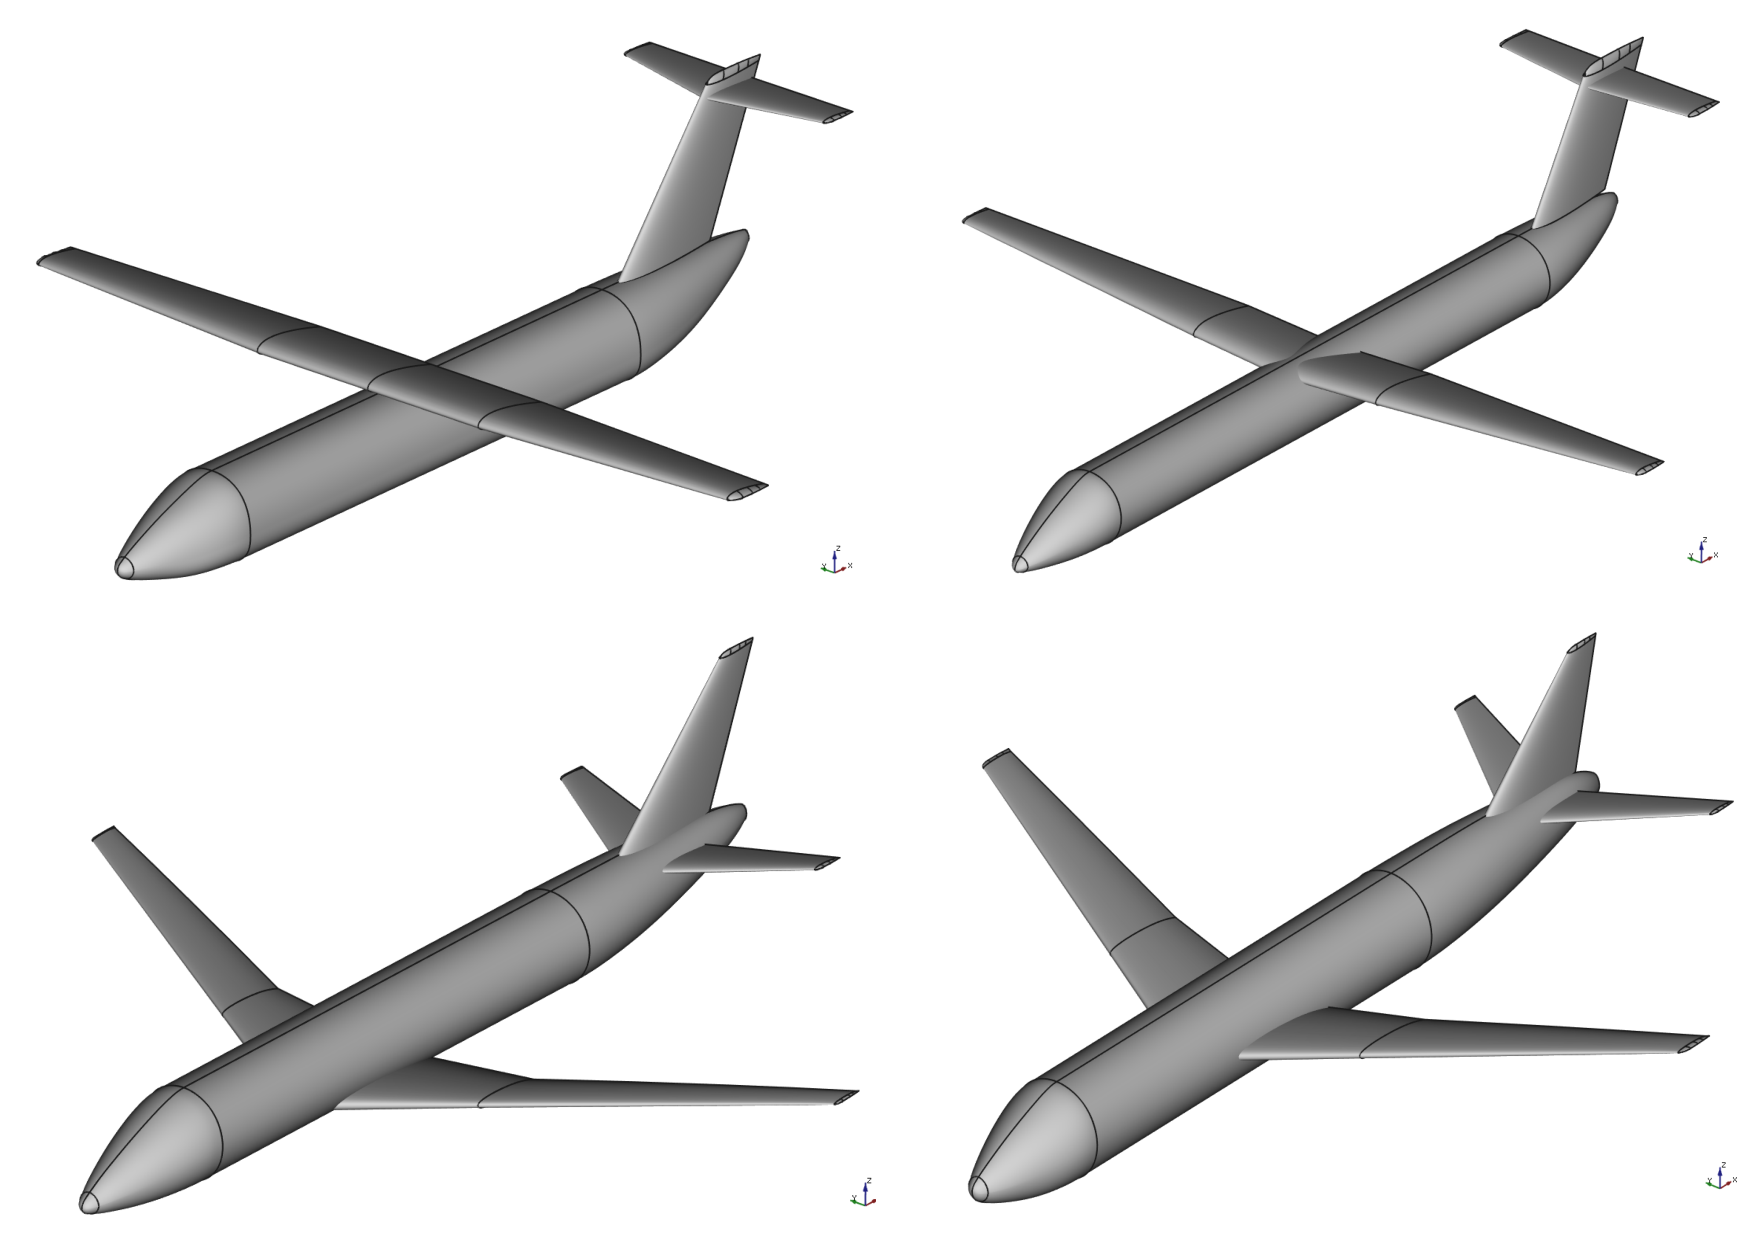
\includegraphics[scale=0.45]{Immagini/Capitolo3/Aircrafts/aircrafts_1}
\caption{Comparison between different aircraft CAD models obtained by using the same test class}
\label{fig:Example01}
\end{figure}
%  
